% =====================================================================
% Báo cáo dự án RoomHub (Booking Classroom) - dựa trên template SOICT
% BIÊN DỊCH BẰNG XeLaTeX (Overleaf: Menu > Compiler > XeLaTeX).
% Bản tối ưu cho Overleaf miễn phí: sơ đồ đã dựng sẵn thành PDF
% (mã nguồn ở Hinhve/nguon_so_do), ảnh đã nén, không dùng TikZ,
% glossaries, subfiles hay BibTeX nên chỉ cần 2 lần biên dịch.
% =====================================================================
\documentclass[a4paper,13pt,twoside]{report}
\usepackage{scrextend}
\changefontsizes{13pt}
\usepackage{iftex}
\ifXeTeX
  \usepackage{fontspec}
  % Nạp font theo tên tệp (nhanh, không cần quét font hệ thống)
  \setmainfont{texgyretermes}[Extension=.otf, UprightFont=*-regular,
    BoldFont=*-bold, ItalicFont=*-italic, BoldItalicFont=*-bolditalic]
  \setmonofont{texgyrecursor}[Scale=0.85, Extension=.otf, UprightFont=*-regular,
    BoldFont=*-bold, ItalicFont=*-italic, BoldItalicFont=*-bolditalic]
\else
  \usepackage[utf8]{vietnam}
  \usepackage{times}
\fi
\usepackage[top=2cm, bottom=2cm, left=3.5cm, right=2.5cm]{geometry}

\usepackage{graphicx}
\usepackage{indentfirst}
\usepackage{array}
\usepackage{enumitem}
\usepackage{titlesec}
\usepackage{titletoc}
\usepackage{chngcntr}
\usepackage{fancyhdr}
\usepackage{appendix}
\usepackage{longtable}
\usepackage{booktabs}
\usepackage{tabularx}
\usepackage{xcolor}
\usepackage[font=small,labelfont=bf]{caption}
\usepackage{float}
\usepackage{subcaption}
\usepackage{xurl}

\usepackage{setspace}
\usepackage{parskip}

\renewcommand\appendixname{PHỤ LỤC}
\renewcommand\appendixpagename{PHỤ LỤC}
\renewcommand\appendixtocname{PHỤ LỤC}


% ----- Định dạng code (fvextra hỗ trợ tiếng Việt trong khối mã) -----
\usepackage{fvextra}
\usepackage{newfloat}
\DeclareFloatingEnvironment[name=Đoạn mã, listname={DANH MỤC ĐOẠN MÃ}, within=chapter]{code}
\captionsetup[code]{skip=4pt}

\fancypagestyle{plain}{%
\fancyhf{}
\fancyfoot[RO,RE]{\thepage}
\renewcommand{\headrulewidth}{0pt}
\renewcommand{\footrulewidth}{0pt}}
\setlength{\headheight}{16pt}

\def \TITLE{BÁO CÁO DỰ ÁN ROOMHUB}
\def \AUTHOR{Nhóm RoomHub}

\titleformat{\chapter}[hang]{\centering\bfseries}{CHƯƠNG \thechapter.\ }{0pt}{}[]
\titlespacing*{\chapter}{0pt}{-20pt}{14pt}
\titleformat{\section}[hang]{\bfseries}{\thechapter.\arabic{section}\ \ \ \ }{0pt}{}[]
\titlespacing{\section}{0pt}{\parskip}{0.5\parskip}
\titleformat{\subsection}[hang]{\bfseries}{\thechapter.\arabic{section}.\arabic{subsection}\ \ \ \ }{0pt}{}[]
\titlespacing{\subsection}{0pt}{\parskip}{0.5\parskip}
\renewcommand\thesubsubsection{\alph{subsubsection}}
\titleformat{\subsubsection}[hang]{\bfseries\itshape}{\alph{subsubsection}, \ }{0pt}{}[]
\titlespacing{\subsubsection}{0pt}{\parskip}{0.3\parskip}

\usepackage{hyperref}
\hypersetup{pdfborder={0 0 0}, pdftitle={\TITLE}, pdfauthor={\AUTHOR}}

\graphicspath{{Hinhve/}}
\counterwithin{figure}{chapter}
\counterwithin{table}{chapter}

\setcounter{secnumdepth}{3}
\setcounter{tocdepth}{2}

\onehalfspacing
\setlength{\parskip}{5pt}
\setlength{\parindent}{15pt}
\setlist{itemsep=1pt,topsep=3pt,parsep=0pt}

% =========================== BODY ===============
\begin{document}
\sloppy\emergencystretch=3em\raggedbottom
\renewcommand{\chaptername}{Chương}\renewcommand{\figurename}{Hình}\renewcommand{\tablename}{Bảng}\renewcommand{\appendixname}{Phụ lục}
\begin{titlepage}
\thispagestyle{empty}
\begin{center}

{\large\bfseries ĐẠI HỌC BÁCH KHOA HÀ NỘI}\par
\vspace{0.15cm}
{\large\bfseries TRƯỜNG ĐIỆN -- ĐIỆN TỬ}\par
\vspace{0.25cm}
{\color{RoomHubBlue}\rule{0.72\textwidth}{1.1pt}}\par

\vspace{2.2cm}
{\Large\bfseries BÁO CÁO GIỮA KỲ}\par
\vspace{0.3cm}
{\large Học phần ET4710 -- Lập trình ứng dụng di động}\par

\vspace{0.7cm}

\includegraphics[width=4.0cm]{Hinhve/logo_roomhub.png}\par
\vspace{0.45cm}
{\color{RoomHubBlue}\bfseries\fontsize{22}{27}\selectfont ROOMHUB}\par
\vspace{0.25cm}
{\Large\bfseries ỨNG DỤNG ĐẶT PHÒNG HỌC VÀ PHÒNG HỌP}\par
\vspace{0.45cm}
{\color{RoomHubBlue}\rule{0.86\textwidth}{0.8pt}}\par

\vspace{1.8cm}
\renewcommand{\arraystretch}{1.35}
\begin{tabular}{>{\bfseries}p{4.1cm}p{6.5cm}r}
Nhóm thực hiện: & Hoàng Văn Tùng & 20252389M \\
                 & Đỗ Thùy Linh & 20252478M \\
                 & Nguyễn Đình Phúc & 20251012M \\
                 & Nguyễn Việt Dũng & 20252690M \\
\addlinespace[0.4cm]
Giảng viên hướng dẫn: & \multicolumn{2}{l}{PGS.TS. Đỗ Trọng Tuấn} \\
\end{tabular}

\vfill
{\small\color{RoomHubGray}\url{https://github.com/xwomen1/classroom-booking}}\par
\vspace{0.75cm}
{\bfseries HÀ NỘI, THÁNG 10 NĂM 2026}

\end{center}
\end{titlepage}


\pagenumbering{roman}
\renewcommand*\contentsname{MỤC LỤC}
\titlecontents{chapter}[0.0cm]{\bfseries\vspace{0.3cm}}{{\bfseries CHƯƠNG \thecontentslabel.\ }}{}{\titlerule*[0.3pc]{.}\contentspage}
\titlecontents{section}[0.0cm]{\vspace{0.15cm}}{\thecontentslabel \ }{}{\titlerule*[0.3pc]{.}\contentspage}
\titlecontents{subsection}[1.0cm]{\vspace{0.1cm}}{\thecontentslabel \ }{}{\titlerule*[0.3pc]{.}\contentspage}
\begingroup\setstretch{1.2}
\tableofcontents
\endgroup
\thispagestyle{empty}

\newpage
\renewcommand{\listfigurename}{DANH MỤC HÌNH VẼ}
{\let\oldnumberline\numberline
\renewcommand{\numberline}{Hình~\oldnumberline}
\listoffigures}

\renewcommand{\listtablename}{DANH MỤC BẢNG BIỂU}
{\let\oldnumberline\numberline
\renewcommand{\numberline}{Bảng~\oldnumberline}
\listoftables}

\chapter*{DANH MỤC THUẬT NGỮ VÀ TỪ VIẾT TẮT}
{\small
\begin{longtable}{|>{\bfseries}p{2.4cm}|p{11.6cm}|}
\hline
\textbf{Thuật ngữ} & \textbf{Ý nghĩa} \\ \hline
\endhead
API & Giao diện lập trình ứng dụng (Application Programming Interface) \\ \hline
APK & Gói cài đặt ứng dụng Android (Android Package) \\ \hline
Booking & Một yêu cầu đặt phòng gồm phòng, ngày, khung giờ và mục đích \\ \hline
CRUD & Tạo, đọc, cập nhật, xóa (Create, Read, Update, Delete) \\ \hline
IoT & Internet vạn vật (Internet of Things) \\ \hline
MQTT & Giao thức truyền thông điệp publish/subscribe (Message Queuing Telemetry Transport) \\ \hline
MVP & Sản phẩm khả dụng tối thiểu (Minimum Viable Product) \\ \hline
No-show & Người đặt không có mặt sử dụng phòng đã được duyệt \\ \hline
PIN & Mã số dùng để mở khóa (Personal Identification Number) \\ \hline
TLS & Giao thức bảo mật tầng vận chuyển (Transport Layer Security) \\ \hline
UAT & Kiểm thử chấp nhận người dùng (User Acceptance Testing) \\ \hline
\end{longtable}
}

\cleardoublepage
\pagenumbering{arabic}
\pagestyle{fancy}
\fancyhf{}
\fancyhead[RE, LO]{\leftmark}
\fancyfoot[RE, LO]{\thepage}

\chapter{GIỚI THIỆU}
\label{chapter:Introduction}
\section{Bối cảnh và bài toán}

Nhu cầu sử dụng phòng học và phòng họp của giảng viên diễn ra thường xuyên, trong khi quy trình đăng ký tại nhiều đơn vị vẫn phụ thuộc vào trao đổi trực tiếp với cán bộ quản lý cơ sở vật chất. Người mượn khó tra cứu nhanh phòng còn trống theo thời gian, sức chứa và thiết bị. Người quản lý cũng phải theo dõi thủ công lịch sử dụng, lịch bảo trì, việc bàn giao chìa khóa hoặc thẻ từ và các trường hợp người đặt không đến.

Các hạn chế trên dễ dẫn đến trùng lịch, lựa chọn phòng không phù hợp và lãng phí tài nguyên. Khi số lượng phòng và lượt đăng ký tăng, việc kiểm tra bằng bảng tính hoặc tin nhắn riêng lẻ không còn bảo đảm tính nhất quán của dữ liệu.

\section{Mục tiêu}

Dự án xây dựng ứng dụng di động \textbf{RoomHub} nhằm quản lý xuyên suốt một lượt mượn phòng, từ tìm kiếm, gửi yêu cầu, phê duyệt đến bàn giao quyền truy cập, sử dụng và kết thúc phiên. Hệ thống hướng tới các mục tiêu sau:

\begin{itemize}
  \item giúp giảng viên tìm và đặt phòng theo tầng, thời gian, sức chứa và thiết bị;
  \item hỗ trợ cán bộ quản lý phê duyệt, đổi phòng, quản lý phòng và lịch bảo trì;
  \item ngăn các trường hợp trùng lịch, vượt giới hạn đặt phòng hoặc đặt vào thời gian bảo trì;
  \item hỗ trợ cả phòng dùng khóa cơ/thẻ từ và phòng dùng khóa mã số;
  \item lưu vết các sự kiện quan trọng như phê duyệt, cấp mã, check-in, check-out và no-show.
\end{itemize}

\section{Phạm vi}

RoomHub phục vụ hai vai trò. \textbf{Quản trị viên} là cán bộ quản lý cơ sở vật chất, có quyền quản lý tài khoản, phòng, yêu cầu đặt phòng, lịch bảo trì, khóa thông minh và các tham số nghiệp vụ. \textbf{Người dùng} là giảng viên, có quyền tìm phòng, tạo và quản lý yêu cầu của mình, thỏa thuận thời gian nhận khóa, tạo mã tạm thời khi được cấp quyền và báo sự cố trong thời gian sử dụng phòng.

Mô hình dữ liệu thử nghiệm gồm tám tầng, mỗi tầng bảy phòng. Mỗi phòng có sức chứa, danh sách thiết bị, trạng thái và một trong hai loại khóa: khóa cơ/thẻ từ hoặc khóa mã số. Với khóa mã số, ứng dụng có thể gửi lệnh tạo PIN tạm thời tới nền tảng OneIoT theo thời gian của lịch đặt.

\section{Định hướng giải pháp và cấu trúc báo cáo}

Ứng dụng Android được phát triển bằng React Native và TypeScript \cite{reactnative}. Ở chế độ cục bộ, dữ liệu được lưu bằng Async Storage \cite{asyncstorage}, cho phép bản Release hoạt động độc lập trên một điện thoại. Dịch vụ Java Spring Boot \cite{springboot} cung cấp REST API và cơ sở dữ liệu H2 để kiểm thử cơ chế đồng bộ. Chế độ dữ liệu được lựa chọn thông qua tham số \texttt{ENABLE\_REMOTE\_SYNC}; bản trình diễn trong báo cáo sử dụng chế độ cục bộ để không phụ thuộc trạng thái của máy chủ.

Đối với phòng dùng khóa mã số, ứng dụng giao tiếp với OneIoT qua MQTT trên TLS \cite{mqtt} và định dạng bản tin oneM2M \cite{onem2m}. Mã PIN được tạo và lưu theo lịch đặt trước khi gửi; khi chưa có kết nối, lệnh được giữ ở trạng thái chờ và được gửi khi phiên kết nối hợp lệ được thiết lập.

Chương \ref{chapter:Implementation} trình bày phạm vi MVP, kiến trúc và tổ chức mã nguồn. Chương \ref{chapter:Testing} mô tả phương pháp kiểm thử và kết quả của phiên bản hiện tại. Phụ lục \ref{appendix:components} chỉ ra vị trí các thành phần chính trong kho mã nguồn; Phụ lục \ref{appendix:prompt} tổng hợp cách nhóm sử dụng trợ lý lập trình và kiểm soát đầu ra.

\chapter{TRIỂN KHAI HỆ THỐNG}
\label{chapter:Implementation}
\section{Tổng quan hệ thống}
\label{section:components}

RoomHub lấy ứng dụng di động làm trung tâm để giảng viên và cán bộ quản lý cùng thực hiện quy trình mượn phòng. Bên cạnh ứng dụng là dịch vụ đồng bộ dữ liệu và các công cụ hỗ trợ kiểm tra giao tiếp với khóa thông minh. Vai trò của từng thành phần được tóm tắt trong Bảng~\ref{tab:components}; vị trí các phần chính trong kho mã nguồn được trình bày tại Phụ lục~\ref{appendix:components}.

\begin{table}[H]
\centering
\caption{Các thành phần chính của hệ thống RoomHub}
\label{tab:components}
\small
\begin{tabularx}{\textwidth}{>{\raggedright\arraybackslash}p{3.4cm} >{\raggedright\arraybackslash}p{2.7cm} X}
\toprule
\rowcolor{RoomHubLight}
\textbf{Thành phần} & \textbf{Công nghệ} & \textbf{Vai trò} \\
\midrule
Ứng dụng di động & React Native, TypeScript, Kotlin & Cung cấp giao diện theo vai trò, xử lý nghiệp vụ, lưu dữ liệu cục bộ và giao tiếp với OneIoT. \\
Dịch vụ đồng bộ & Java, Spring Boot, H2 & Cung cấp giao diện dữ liệu cho tài khoản, phòng, lịch đặt, bảo trì, quyền truy cập và thông báo. \\
Mô phỏng khóa thông minh & Python & Tạo môi trường kiểm tra bản tin cấp mật khẩu và sự kiện truy cập khi chưa dùng khóa vật lý. \\
Công cụ giao tiếp & Python, MQTT & Làm mẫu tham chiếu cho cơ chế kết nối và định dạng bản tin trao đổi với OneIoT. \\
\bottomrule
\end{tabularx}
\end{table}

Hình~\ref{fig:architecture} thể hiện quan hệ giữa các thành phần. Trong ứng dụng, màn hình tiếp nhận thao tác của người dùng; lớp nghiệp vụ kiểm tra quyền và quy tắc đặt phòng; lớp lưu trữ giữ dữ liệu cục bộ hoặc trao đổi với dịch vụ đồng bộ theo chế độ hoạt động.

\begin{figure}[H]
\centering
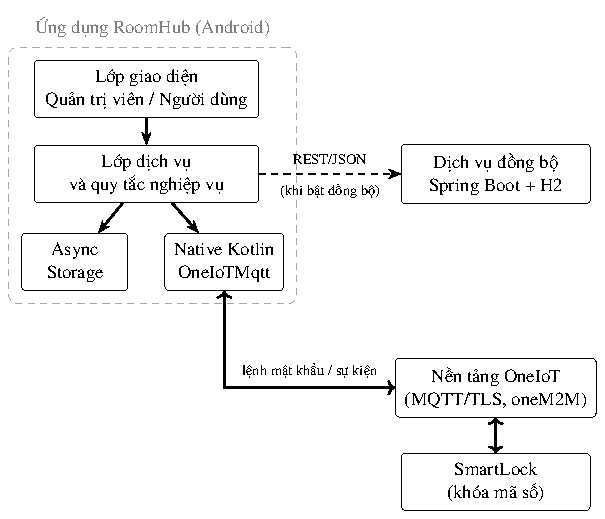
\includegraphics[width=0.78\textwidth]{kien_truc.pdf}
\caption{Kiến trúc tổng thể của hệ thống RoomHub}
\label{fig:architecture}
\end{figure}

\section{Phạm vi sản phẩm khả dụng tối thiểu}
\label{section:mvp}

Phạm vi sản phẩm khả dụng tối thiểu là thực hiện trọn luồng mượn phòng trên một điện thoại Android: tìm phòng, gửi yêu cầu, phê duyệt, sử dụng và kết thúc. Ứng dụng có bản cài đặt chạy độc lập, còn các quy tắc nghiệp vụ chính được kiểm tra bằng ca kiểm thử tương ứng. Bảng~\ref{tab:mvp} phân biệt chức năng đã triển khai với phần cần kiểm chứng thêm trên nhiều thiết bị hoặc với khóa thật.

\begin{table}[H]
\centering
\caption{Phạm vi sản phẩm khả dụng tối thiểu}
\label{tab:mvp}
\small
\begin{tabularx}{\textwidth}{>{\raggedright\arraybackslash}p{3.4cm} X >{\centering\arraybackslash}p{1.9cm}}
\toprule
\rowcolor{RoomHubLight}
\textbf{Nhóm chức năng} & \textbf{Nội dung} & \textbf{Trạng thái} \\
\midrule
Tài khoản & Đăng nhập, đăng ký, đổi hoặc khôi phục mật khẩu, hồ sơ và quyền quản trị tài khoản. & Đã triển khai \\
Tìm phòng & Lọc theo tầng, thời gian, sức chứa, thiết bị và loại khóa; xem sơ đồ phòng theo trạng thái. & Đã triển khai \\
Đặt và duyệt & Tạo yêu cầu, kiểm tra quy tắc; phê duyệt, từ chối, đổi phòng và hủy theo thời hạn. & Đã triển khai \\
Đặt lặp hàng tuần & Tạo tối đa tám lượt, quản lý các lượt tương lai và duyệt theo chuỗi. & Đã triển khai \\
Phòng và bảo trì & Quản lý thông tin phòng, lịch bảo trì, yêu cầu báo sự cố và lịch sử sử dụng. & Đã triển khai \\
Truy cập phòng & Thỏa thuận lịch nhận khóa cơ/thẻ từ; cấp quyền và tạo mã PIN bảy chữ số cho phòng khóa số. & Đã triển khai \\
Điểm danh & Ghi nhận việc vào, ra phòng và xử lý trường hợp người đặt không đến. & Đã triển khai \\
Thông báo, cấu hình & Thông báo theo sự kiện, thông báo ưu tiên và điều chỉnh quy tắc nghiệp vụ. & Đã triển khai \\
\midrule
Đồng bộ nhiều thiết bị & Dùng dịch vụ dữ liệu chung; hiện đã kiểm tra với máy chủ và cơ sở dữ liệu trong môi trường cục bộ. & Đang hoàn thiện \\
Kiểm chứng khóa thật & Xác nhận khóa vật lý nhận và áp dụng mật khẩu theo đúng thời hạn. & Giai đoạn sau \\
Chức năng mở rộng & Thống kê mức sử dụng, gợi ý phòng nâng cao và phương án điểm danh bổ sung. & Giai đoạn sau \\
\bottomrule
\end{tabularx}
\end{table}

Quản trị viên có thể điều chỉnh khoảng thời gian được phép đặt trước. Cấu hình ban đầu cho phép đặt trước từ một đến ba ngày; nếu cho phép đặt cùng ngày, giới hạn tối thiểu có thể giảm về không. Tổng số yêu cầu đang chờ xử lý và lượt đã duyệt sắp sử dụng của mỗi người dùng không vượt quá hai. Việc hủy và đổi phòng phải tuân theo thời hạn trước giờ bắt đầu. Với khóa số, mã PIN có hiệu lực từ mười phút trước giờ bắt đầu đến mười phút sau giờ kết thúc. Nếu chưa có check-in sau thời gian chờ mặc định mười lăm phút kể từ giờ bắt đầu, quản trị viên có thể xác nhận vắng mặt. Các mốc thời gian này được kiểm tra theo cấu hình hiện hành. Vòng đời một lượt đặt phòng được minh họa ở Hình~\ref{fig:state}.

\begin{figure}[H]
\centering
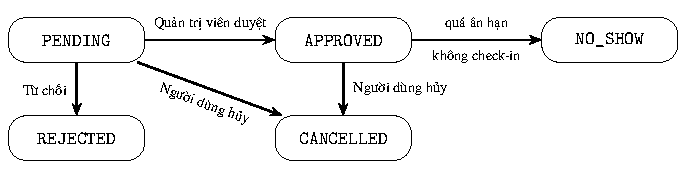
\includegraphics[width=0.98\textwidth]{trang_thai_booking.pdf}
\caption{Vòng đời trạng thái của một lượt đặt phòng}
\label{fig:state}
\end{figure}

\section{Tổ chức và phân chia trách nhiệm}

Mã nguồn ứng dụng được chia thành phần hạ tầng dùng chung, các thành phần giao diện tái sử dụng và mười module nghiệp vụ. Mỗi module tập hợp màn hình, dịch vụ xử lý và mô hình dữ liệu của một phạm vi chức năng. Cách tổ chức này giúp các thành viên phụ trách những phần khác nhau mà vẫn dùng chung quy tắc về tài khoản, lưu trữ và trao đổi dữ liệu.

Khi hoạt động cục bộ, thao tác nghiệp vụ đọc và ghi dữ liệu trên điện thoại. Ở chế độ đồng bộ, ứng dụng trao đổi dữ liệu với máy chủ qua giao diện mạng và sử dụng phiên đăng nhập để xác định quyền truy cập. Hai chế độ cùng phục vụ một luồng thao tác của người dùng; việc kiểm chứng trên nhiều thiết bị vẫn là công việc tiếp theo.

\section{Các module nghiệp vụ}
\label{section:modules}

Bảng~\ref{tab:modules} trình bày trách nhiệm của mười module nghiệp vụ. Các mục tiếp theo giải thích cách chúng phối hợp trong những luồng chính của ứng dụng.

\begin{table}[H]
\centering
\caption{Phân chia module của ứng dụng}
\label{tab:modules}
\small
\begin{tabularx}{\textwidth}{>{\raggedright\arraybackslash}p{4.1cm} X}
\toprule
\rowcolor{RoomHubLight}
\textbf{Module} & \textbf{Trách nhiệm chính} \\
\midrule
Xác thực & Đăng nhập, đăng ký, đổi và khôi phục mật khẩu. \\
Quản lý tài khoản & Tìm kiếm, cập nhật, phân quyền và vô hiệu hóa tài khoản. \\
Quản lý phòng & Lưu thông tin phòng, tìm kiếm và trình bày sơ đồ theo tầng. \\
Đặt phòng & Tạo, duyệt, hủy, đổi phòng, đặt lặp và theo dõi việc sử dụng. \\
Lịch và bảo trì & Quản lý lịch bảo trì, tiếp nhận yêu cầu báo sự cố. \\
Quyền truy cập & Cấp quyền theo phòng và tạo mã PIN tạm thời. \\
Khóa thông minh & Gắn khóa vào phòng, trao đổi bản tin và tiếp nhận sự kiện từ khóa. \\
Thông báo & Gửi và phân loại thông báo theo sự kiện nghiệp vụ. \\
Hồ sơ cá nhân & Xem và cập nhật thông tin của người đang đăng nhập. \\
Cấu hình & Điều chỉnh giới hạn đặt phòng và các thời hạn nghiệp vụ. \\
\bottomrule
\end{tabularx}
\end{table}

\subsection{Tài khoản và quản lý người dùng}

Lần chạy đầu, ứng dụng chuẩn bị hai tài khoản thử nghiệm tương ứng với hai vai trò. Khi đăng ký, người dùng phải nhập tên đăng nhập, mật khẩu và xác nhận mật khẩu; thông tin cá nhân và mã khôi phục là tùy chọn. Hệ thống từ chối tên đăng nhập trùng hoặc mật khẩu không hợp lệ. Việc khôi phục mật khẩu chỉ áp dụng cho tài khoản đã thiết lập mã khôi phục.

Trước những thao tác có ảnh hưởng đến dữ liệu, ứng dụng kiểm tra tài khoản còn hoạt động và có đúng quyền. Quản trị viên không thể tự vô hiệu hóa hoặc xóa tài khoản của mình, đồng thời không thể xóa tài khoản còn lịch đặt đang hoạt động.

\subsection{Phòng và tra cứu phòng}

Dữ liệu trình diễn gồm 56 phòng thuộc tám tầng, mỗi tầng bảy phòng với sức chứa và thiết bị khác nhau. Khi thêm hoặc sửa phòng, hệ thống kiểm tra tầng, sức chứa và tên phòng để tránh dữ liệu không hợp lệ hoặc trùng lặp. Phòng còn gắn với yêu cầu đang hoạt động không được xóa.

Giảng viên có thể lọc phòng theo tầng, khung giờ, sức chứa, thiết bị và loại khóa. Kết quả được thể hiện trên sơ đồ tầng với màu trạng thái. Ở phía quản trị, danh sách phòng được thu gọn theo tám tầng; chọn một phòng sẽ mở các thao tác sửa, xóa, lên lịch bảo trì và xem lịch sử sử dụng.

\subsection{Đặt phòng, phê duyệt và sử dụng}

Khi gửi yêu cầu, ứng dụng kiểm tra phòng còn hoạt động, mục đích sử dụng đã được nhập, thời gian nằm trong khoảng được phép đặt và phiên sử dụng chưa kết thúc. Yêu cầu bị từ chối nếu phòng đang bảo trì, đã có lịch trùng, người đặt có lịch sử dụng khác cùng thời điểm hoặc đã đạt giới hạn yêu cầu. Hai lịch được xem là trùng khi cùng phòng và khoảng thời gian sử dụng của chúng có phần giao nhau; các khoảng chỉ tiếp giáp ở thời điểm kết thúc hoặc bắt đầu vẫn có thể được xét riêng.

Với yêu cầu lặp hàng tuần, hệ thống tạo tối đa tám lượt và kiểm tra cả chuỗi trước khi ghi nhận. Nếu một lượt vi phạm quy tắc, thao tác không được lưu dở dang. Quản trị viên duyệt hoặc từ chối yêu cầu sau khi kiểm tra lại lịch phòng và lịch bảo trì. Khi cần đổi phòng, phòng thay thế phải có cùng loại khóa, sức chứa không nhỏ hơn và đủ thiết bị so với phòng ban đầu.

Lịch sắp tới, lịch đã sử dụng và lịch đã hủy được trình bày theo trạng thái để tránh lặp thao tác ở nhiều nơi. Nếu đã hết thời gian chờ check-in mà vẫn chưa có bằng chứng vào phòng, quản trị viên có thể ghi nhận vắng mặt; khung giờ được giải phóng và quyền dùng mã tương ứng được thu hồi.

\subsection{Bảo trì và báo sự cố}

Quản trị viên có thể tạo lịch bảo trì cố định, nhưng lịch này không được chồng với bảo trì khác hoặc lượt đặt đã được duyệt. Nếu phòng đã được đặt, người quản lý phải xử lý việc đổi phòng trước khi chặn sử dụng. Trong thời gian sử dụng phòng theo một lượt đặt đã duyệt, người dùng có thể báo sự cố tại phòng và nêu lý do. Mỗi lượt sử dụng chỉ có một yêu cầu báo sự cố đang chờ xử lý; tầng và phòng liên quan được đánh dấu để quản trị viên nhận biết.

\subsection{Quyền truy cập và khóa thông minh}

Quyền tự tạo mã PIN được cấp theo từng cặp người dùng và phòng. Vì vậy, việc thu hồi quyền ở một phòng không làm thay đổi quyền ở phòng khác. Trước khi cấp mã, hệ thống đối chiếu lịch đã duyệt, người sở hữu lịch, loại khóa, thời hạn sử dụng và quyền tại phòng. Mỗi mã có bảy chữ số và thời hạn bao gồm mười phút trước giờ bắt đầu đến mười phút sau giờ kết thúc.

Ứng dụng lưu mã để người dùng nhìn thấy trước. Nếu đã có phiên kết nối OneIoT, lệnh tạo mật khẩu được gửi đến khóa gắn với phòng; nếu chưa kết nối, lệnh được giữ chờ và gửi khi phiên hợp lệ được mở. Cách xử lý này cho phép chuẩn bị mã trong lúc mất mạng, nhưng việc khóa thật nhận và áp dụng mã vẫn cần kiểm chứng riêng. Với phòng dùng khóa cơ hoặc thẻ từ, người dùng và quản trị viên thống nhất lịch nhận khóa; người dùng có thể ủy quyền người nhận hộ theo quy định.

Ứng dụng cũng tiếp nhận sự kiện truy cập do khóa phát ra để cập nhật việc vào và ra phòng. Thông tin xác thực OneIoT chỉ tồn tại trong phiên làm việc và được xóa khi phiên kết thúc.

\subsection{Thông báo, hồ sơ và cấu hình}

Các sự kiện như gửi yêu cầu, duyệt, từ chối, cấp mã hoặc đổi phòng đều tạo thông báo. Màu sắc thể hiện tính chất tích cực, tiêu cực, cần chú ý hoặc trung tính của từng sự kiện. Thông báo ưu tiên có thể được hiển thị nổi. Người dùng quản lý hồ sơ cá nhân; quản trị viên điều chỉnh các giới hạn và thời hạn nghiệp vụ. Trước khi lưu cấu hình, hệ thống kiểm tra các giá trị không âm, khoảng đặt trước hợp lệ và giới hạn yêu cầu tối thiểu là một.

\subsection{Dịch vụ đồng bộ dữ liệu}

Dịch vụ Java Spring Boot cung cấp giao diện dữ liệu cho tài khoản, phòng, cấu hình, bảo trì, lịch đặt, quyền tạo mã và thông báo. Máy chủ xác thực phiên, kiểm tra quy tắc nghiệp vụ và trả lỗi theo cùng một định dạng. Cơ sở dữ liệu H2 được dùng để kiểm thử cục bộ; cấu hình kết nối cơ sở dữ liệu từ xa đã được chuẩn bị. Bản trình diễn trên điện thoại dùng dữ liệu cục bộ để không phụ thuộc trạng thái máy chủ.

\section{Điều hướng giao diện}

Hình~\ref{fig:ui-flow} tóm tắt cách di chuyển giữa các chức năng theo vai trò. Giảng viên chọn khung giờ, lọc và chọn phòng, nhập mục đích rồi gửi yêu cầu ngay trên cùng một màn hình. Quản trị viên mở quản lý phòng và bảo trì theo tầng, chọn phòng rồi thực hiện thao tác tương ứng. Các chức năng khác được mở từ màn hình chính của từng vai trò. Các màn hình tương ứng được trình bày ngay sau sơ đồ điều hướng.

\begin{figure}[H]
\centering
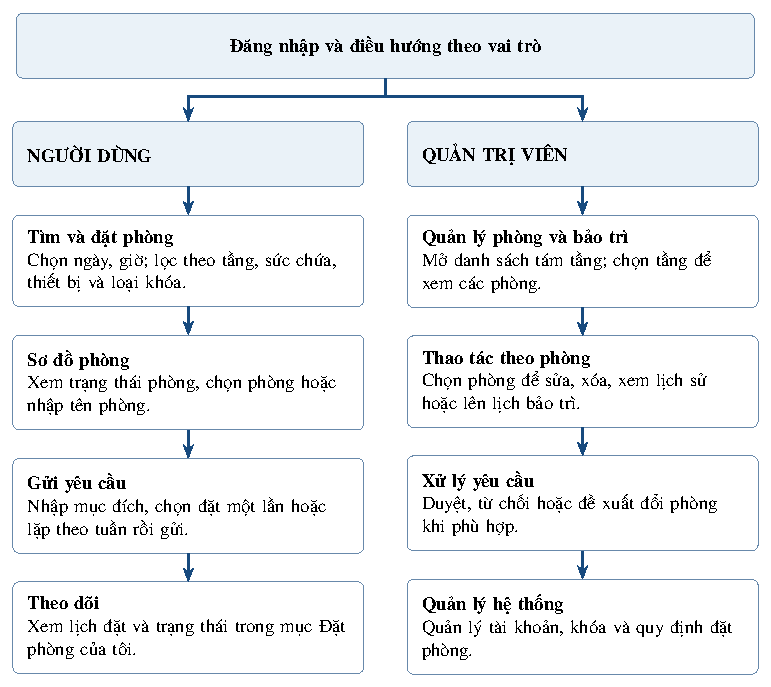
\includegraphics[width=0.95\textwidth]{dieu_huong_giao_dien.pdf}
\caption{Luồng điều hướng giao diện theo hai vai trò}
\label{fig:ui-flow}
\end{figure}

\clearpage
\section{Giao diện ứng dụng hiện tại}
Các ảnh dưới đây được chụp trực tiếp từ phiên bản ứng dụng hiện tại cài trên điện thoại Android. Chúng minh họa màn hình theo vai trò, thao tác tìm và đặt phòng trên cùng một màn hình, cùng cách quản lý phòng theo tầng đã nêu ở Hình~\ref{fig:ui-flow}.

\begin{figure}[H]
\centering
\begin{subfigure}[t]{0.43\textwidth}
  \centering
  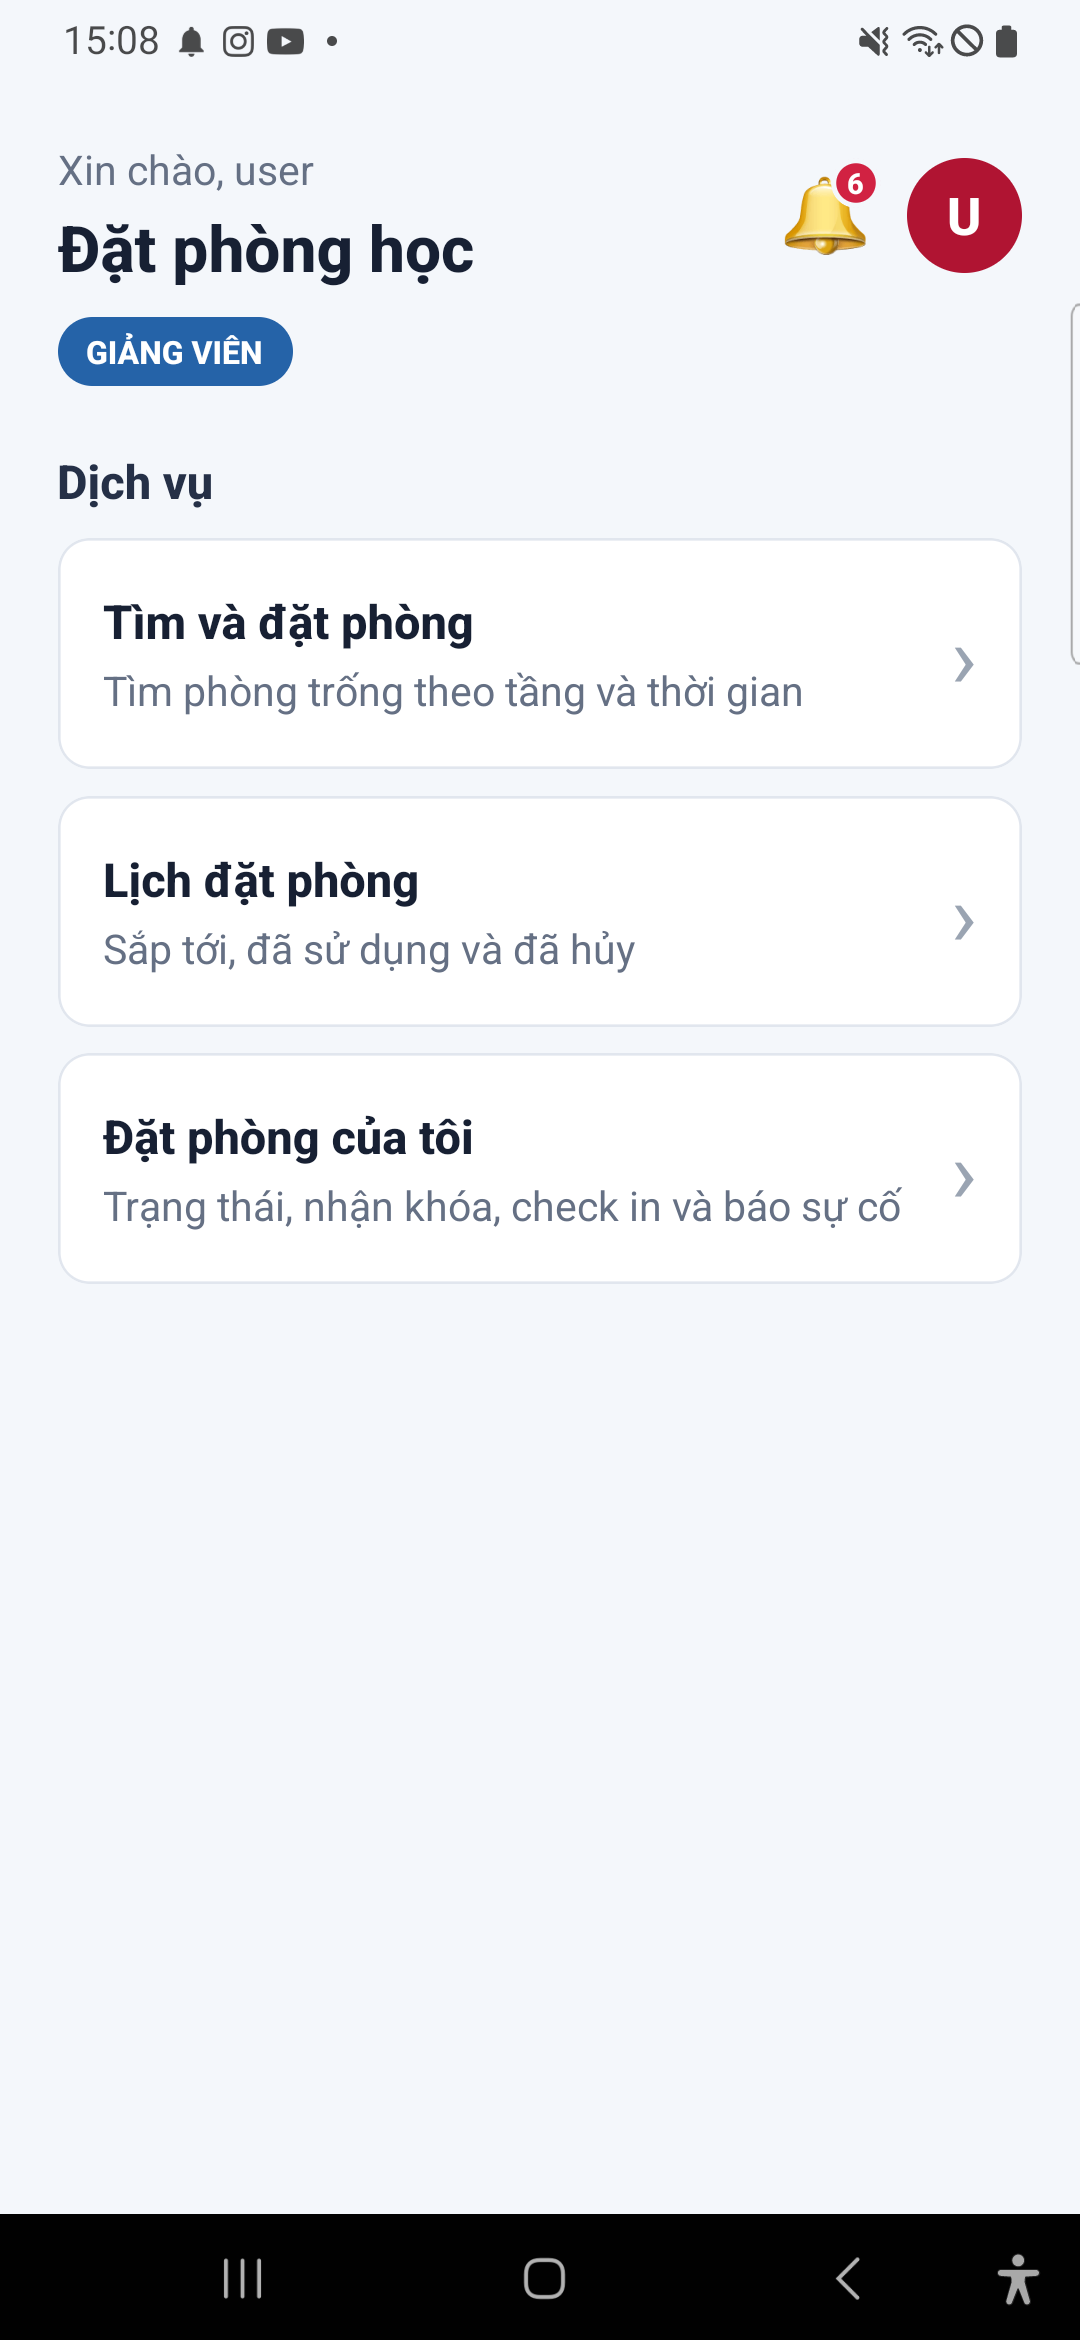
\includegraphics[width=\linewidth]{giao_dien_nguoi_dung_hien_tai.png}
  \caption{Màn hình người dùng}
\end{subfigure}
\hfill
\begin{subfigure}[t]{0.43\textwidth}
  \centering
  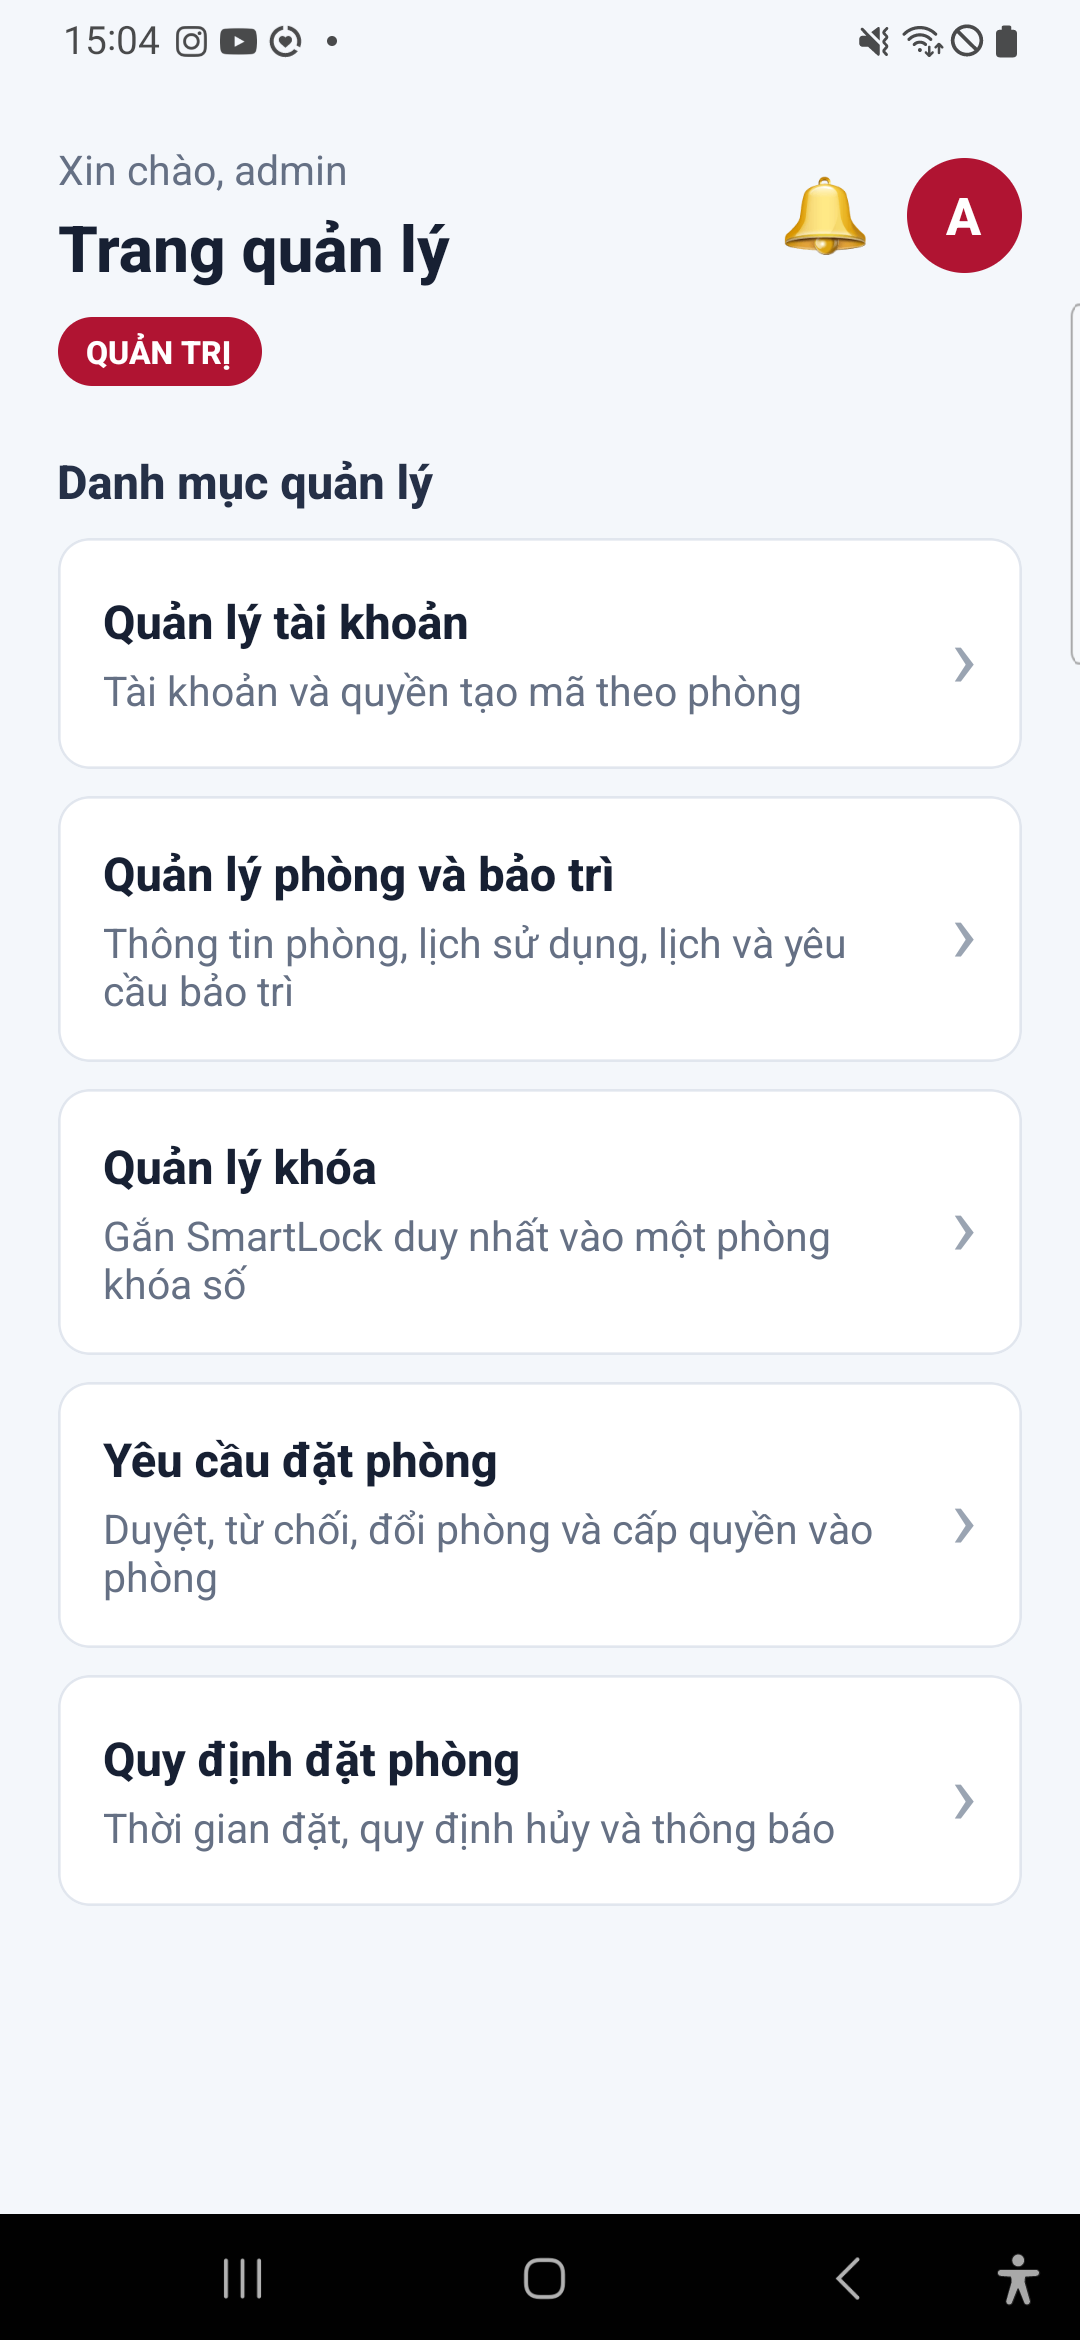
\includegraphics[width=\linewidth]{giao_dien_admin_hien_tai.png}
  \caption{Màn hình quản trị viên}
\end{subfigure}
\caption{Màn hình chính theo hai vai trò của ứng dụng hiện tại}
\label{fig:current-dashboards}
\end{figure}

\begin{figure}[H]
\centering
\begin{subfigure}[t]{0.43\textwidth}
  \centering
  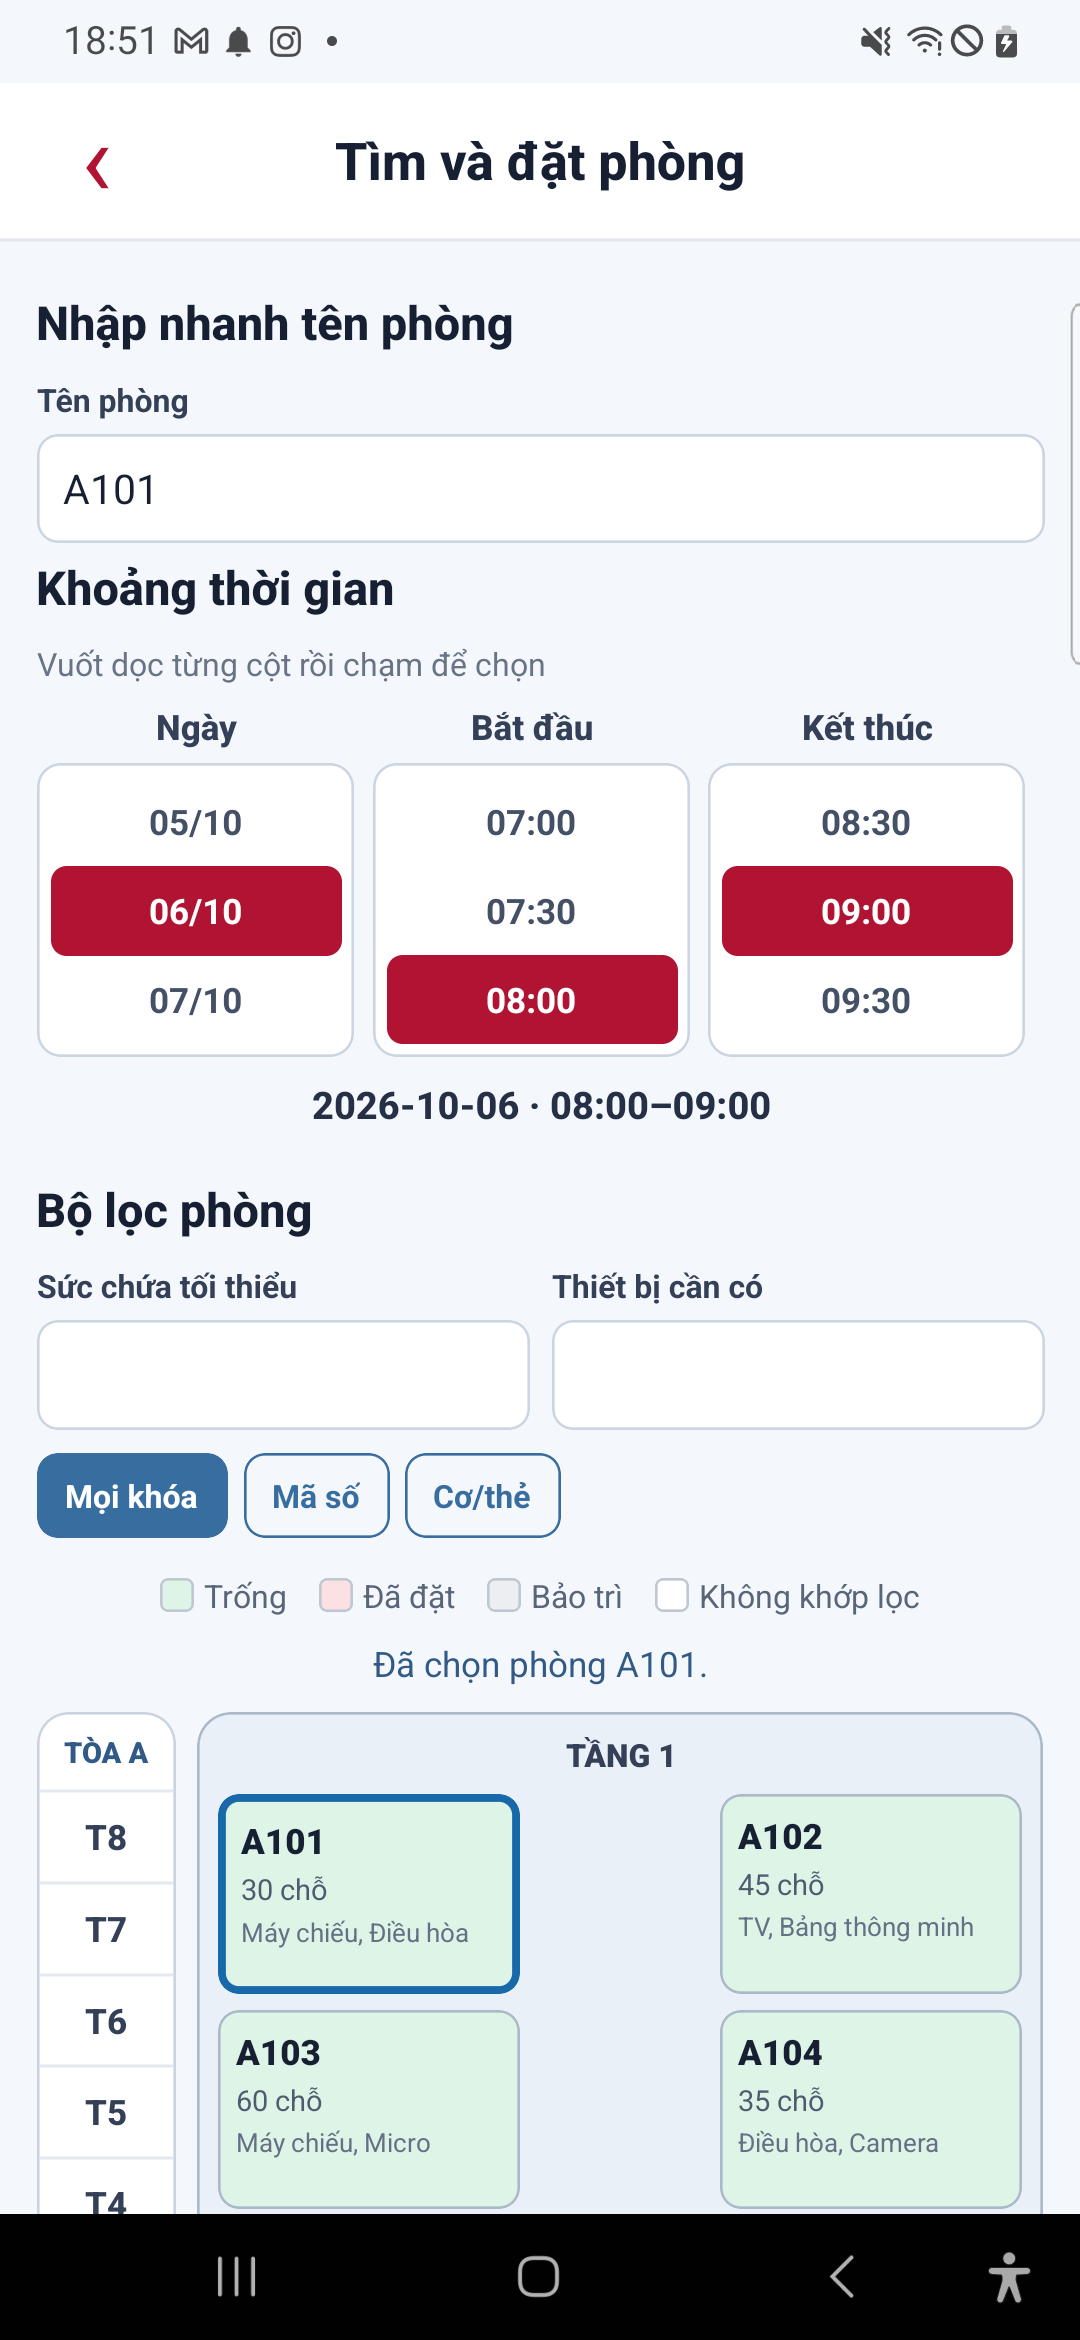
\includegraphics[width=\linewidth]{tim_va_dat_phong_hien_tai.png}
  \caption{Chọn thời gian và lọc phòng}
\end{subfigure}
\hfill
\begin{subfigure}[t]{0.43\textwidth}
  \centering
  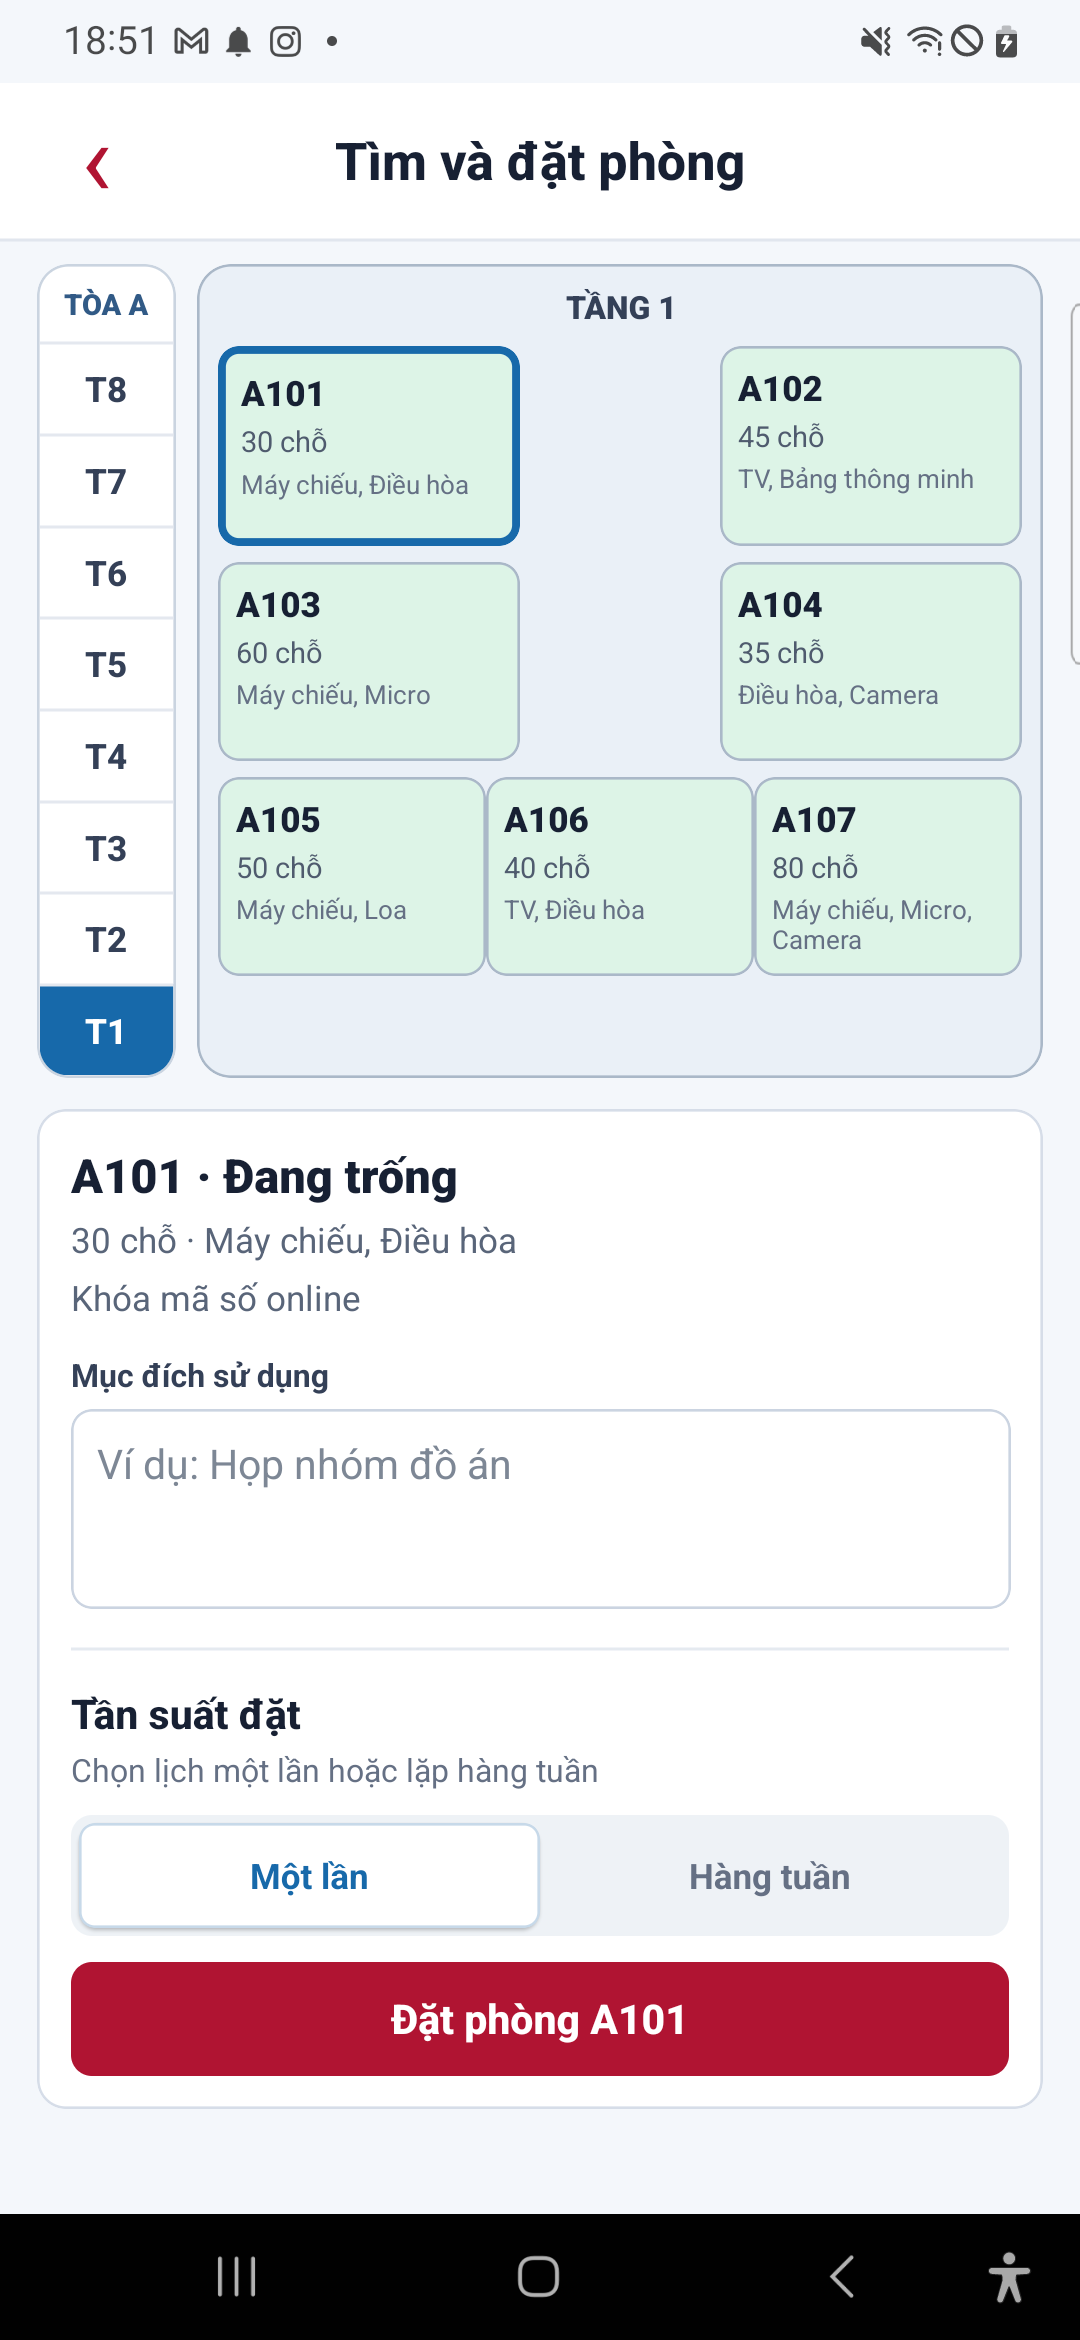
\includegraphics[width=\linewidth]{chon_phong_va_dat_hien_tai.png}
  \caption{Chọn phòng và nhập thông tin đặt}
\end{subfigure}
\caption{Tìm phòng và tạo yêu cầu trên cùng một màn hình}
\label{fig:current-booking}
\end{figure}

\begin{figure}[H]
\centering
\begin{subfigure}[t]{0.43\textwidth}
  \centering
  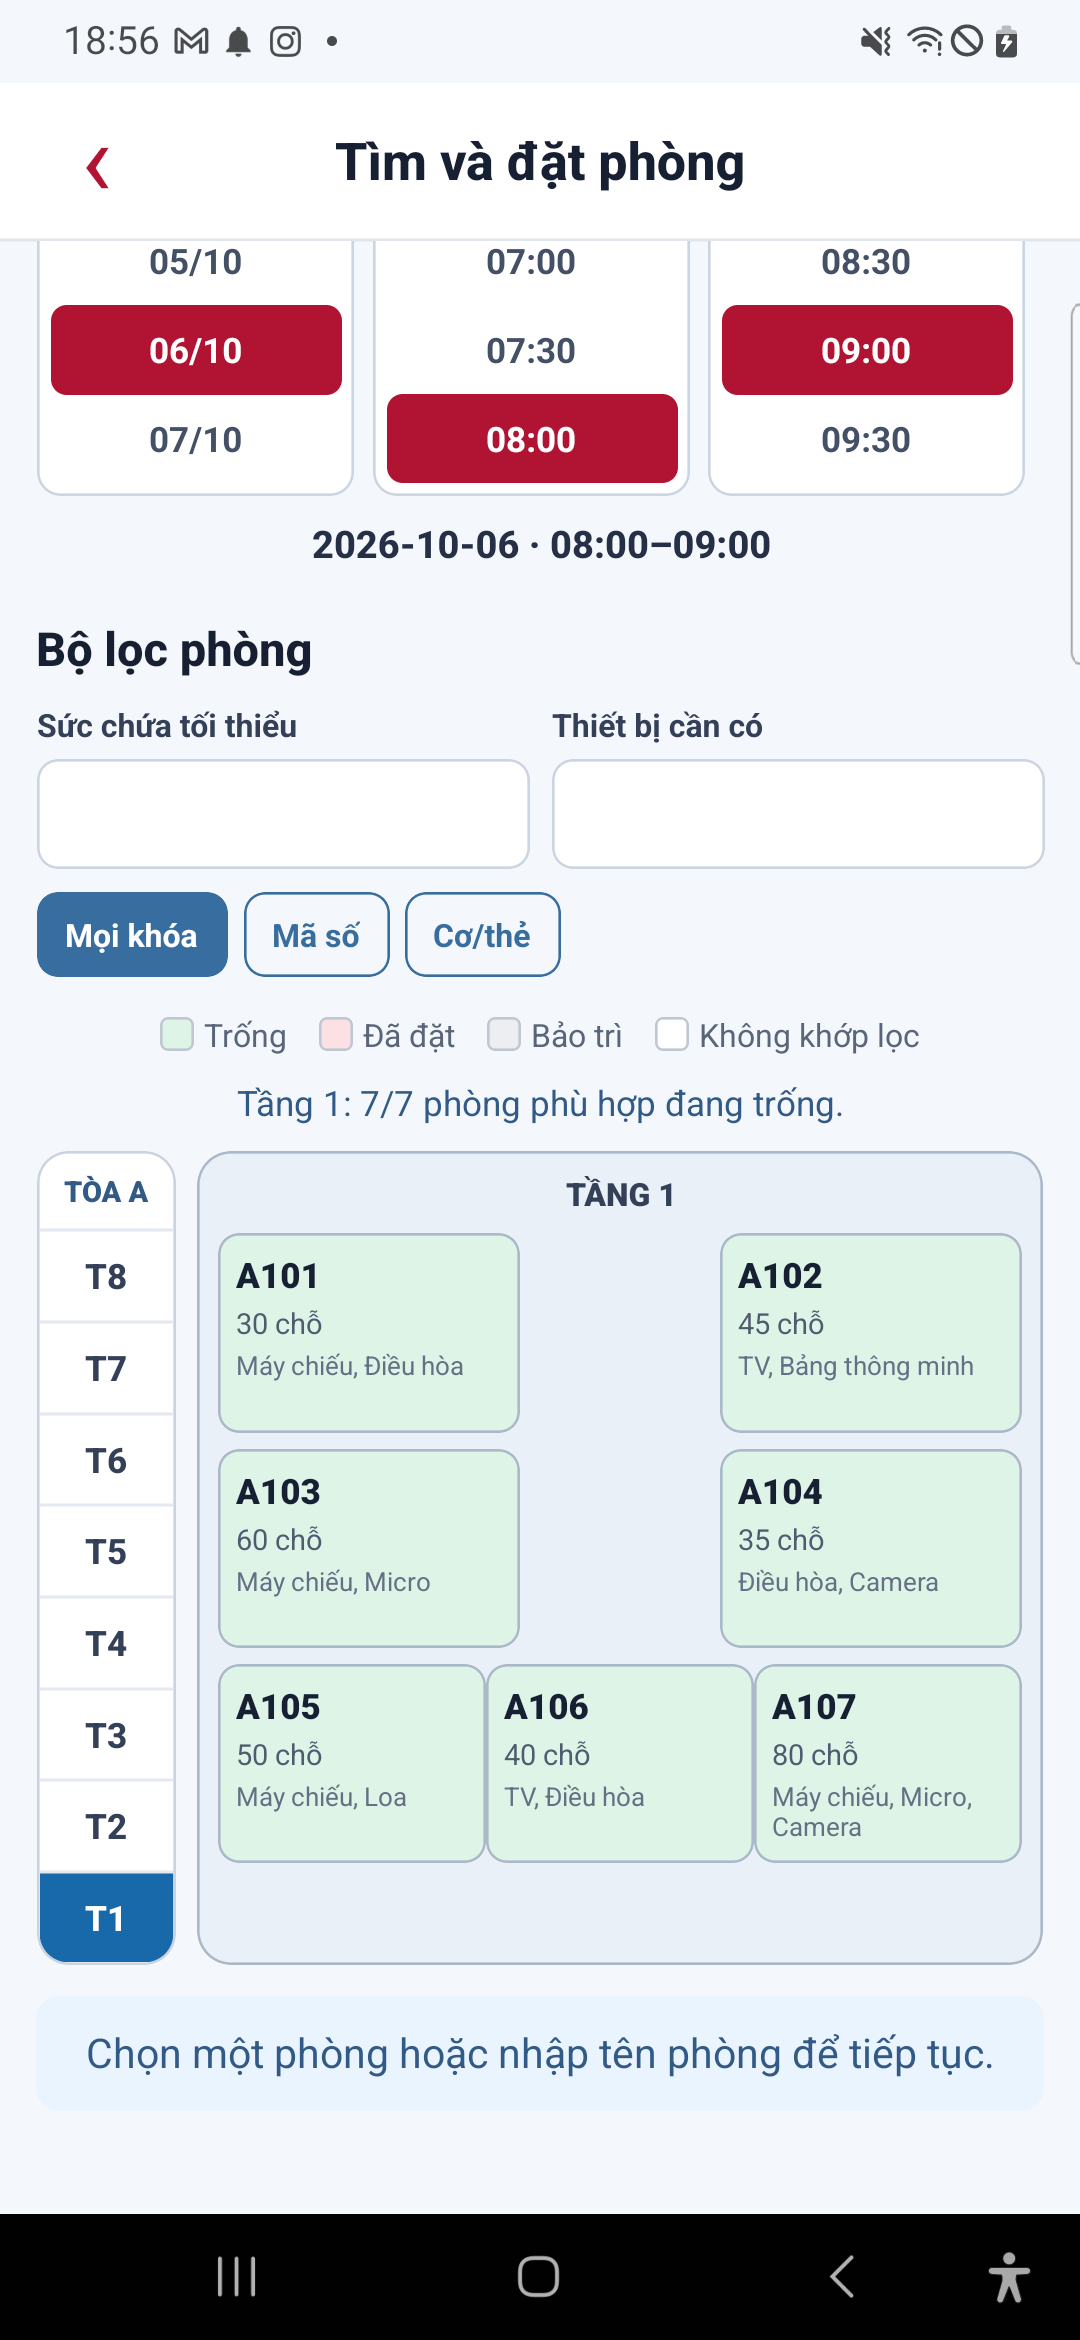
\includegraphics[width=\linewidth]{so_do_phong_hien_tai.png}
  \caption{Sơ đồ phòng theo tầng}
\end{subfigure}
\hfill
\begin{subfigure}[t]{0.43\textwidth}
  \centering
  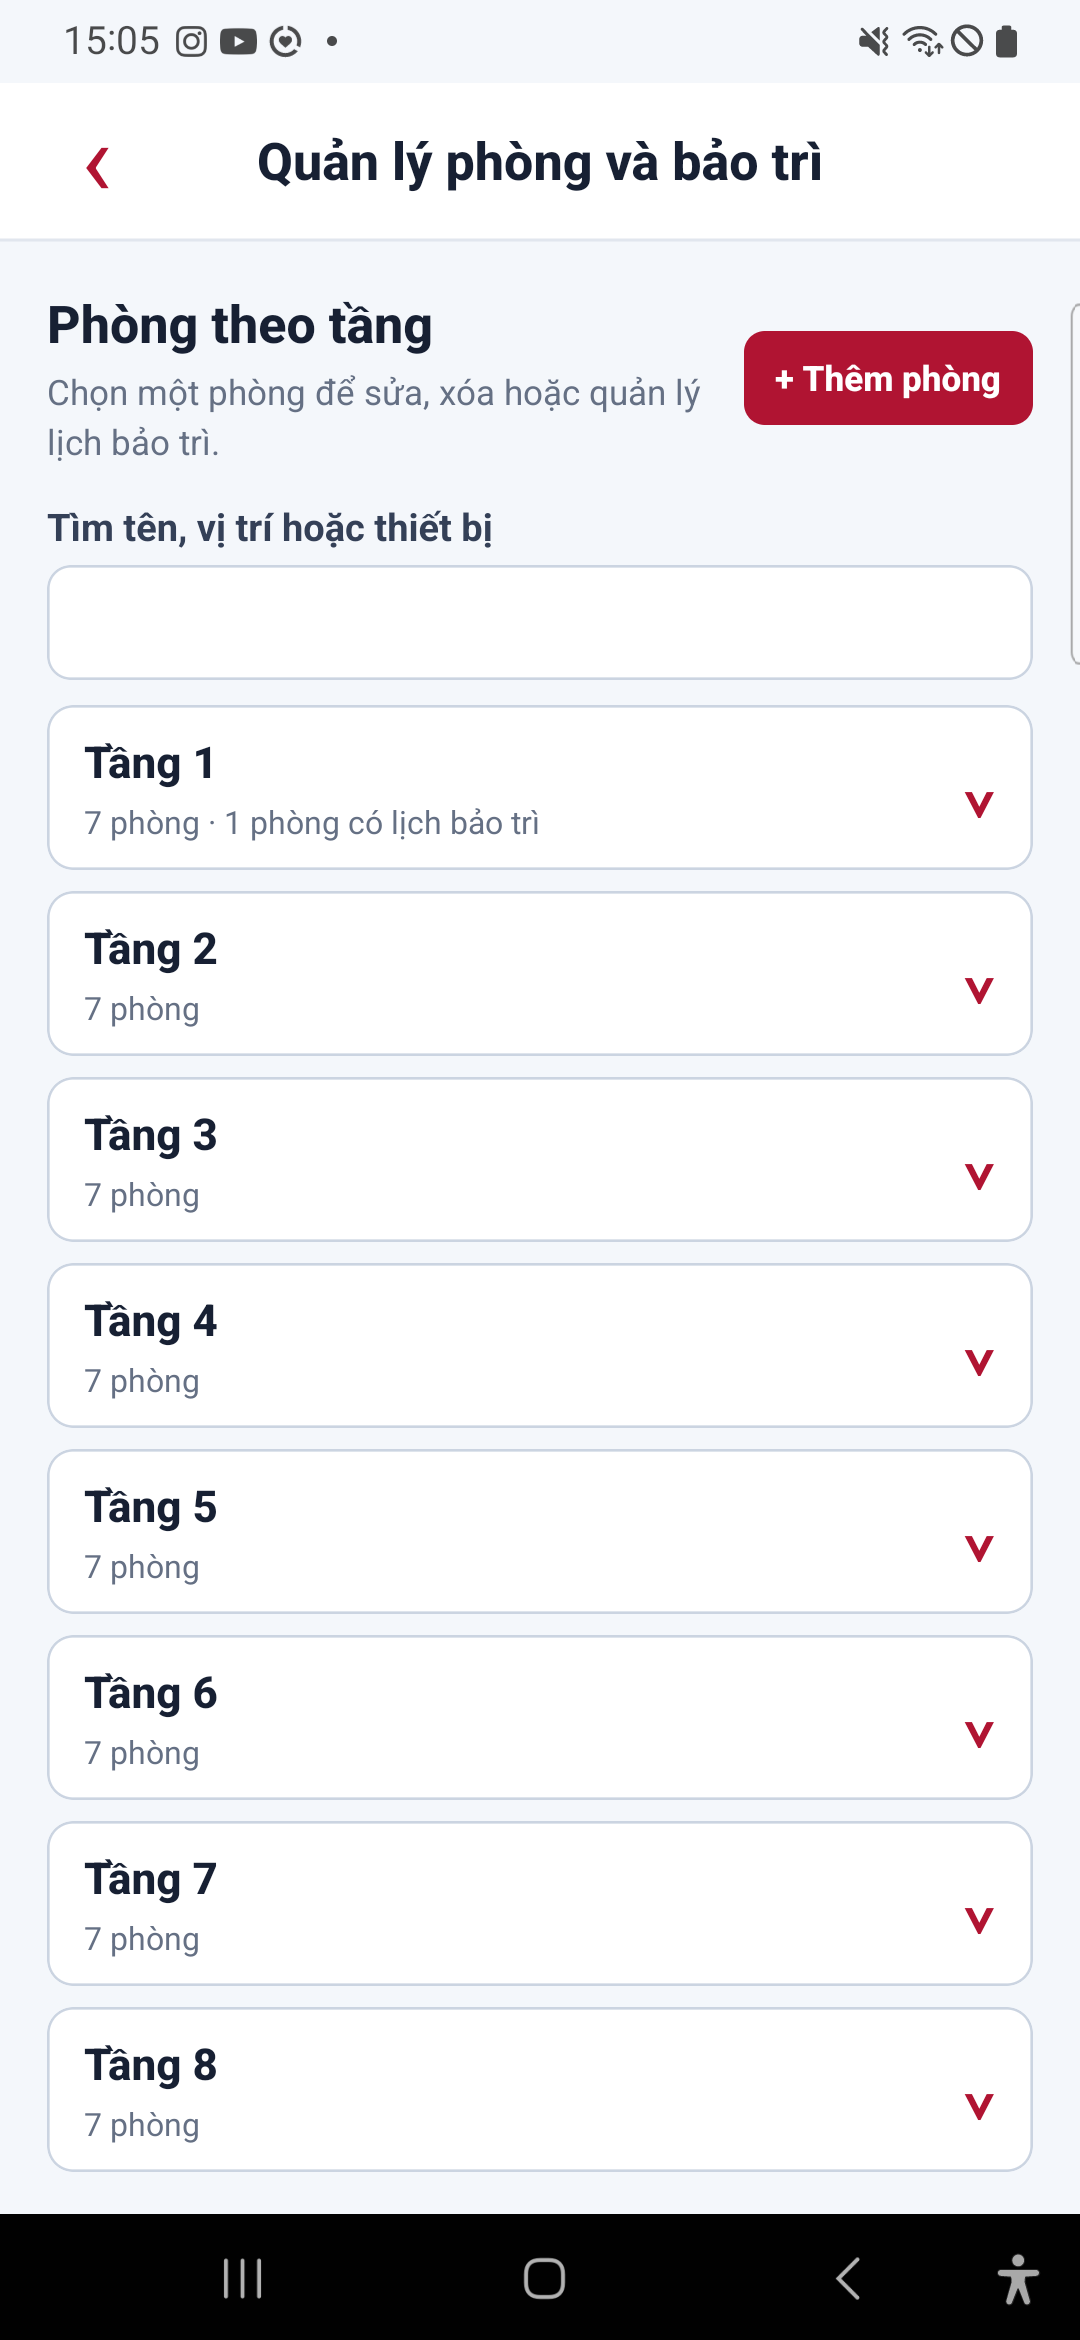
\includegraphics[width=\linewidth]{quan_ly_phong_theo_tang_hien_tai.png}
  \caption{Danh sách tầng của quản trị viên}
\end{subfigure}
\caption{Hai cách xem phòng theo tầng ở ứng dụng hiện tại}
\label{fig:current-floors}
\end{figure}

\begin{figure}[H]
\centering
\begin{subfigure}[t]{0.43\textwidth}
  \centering
  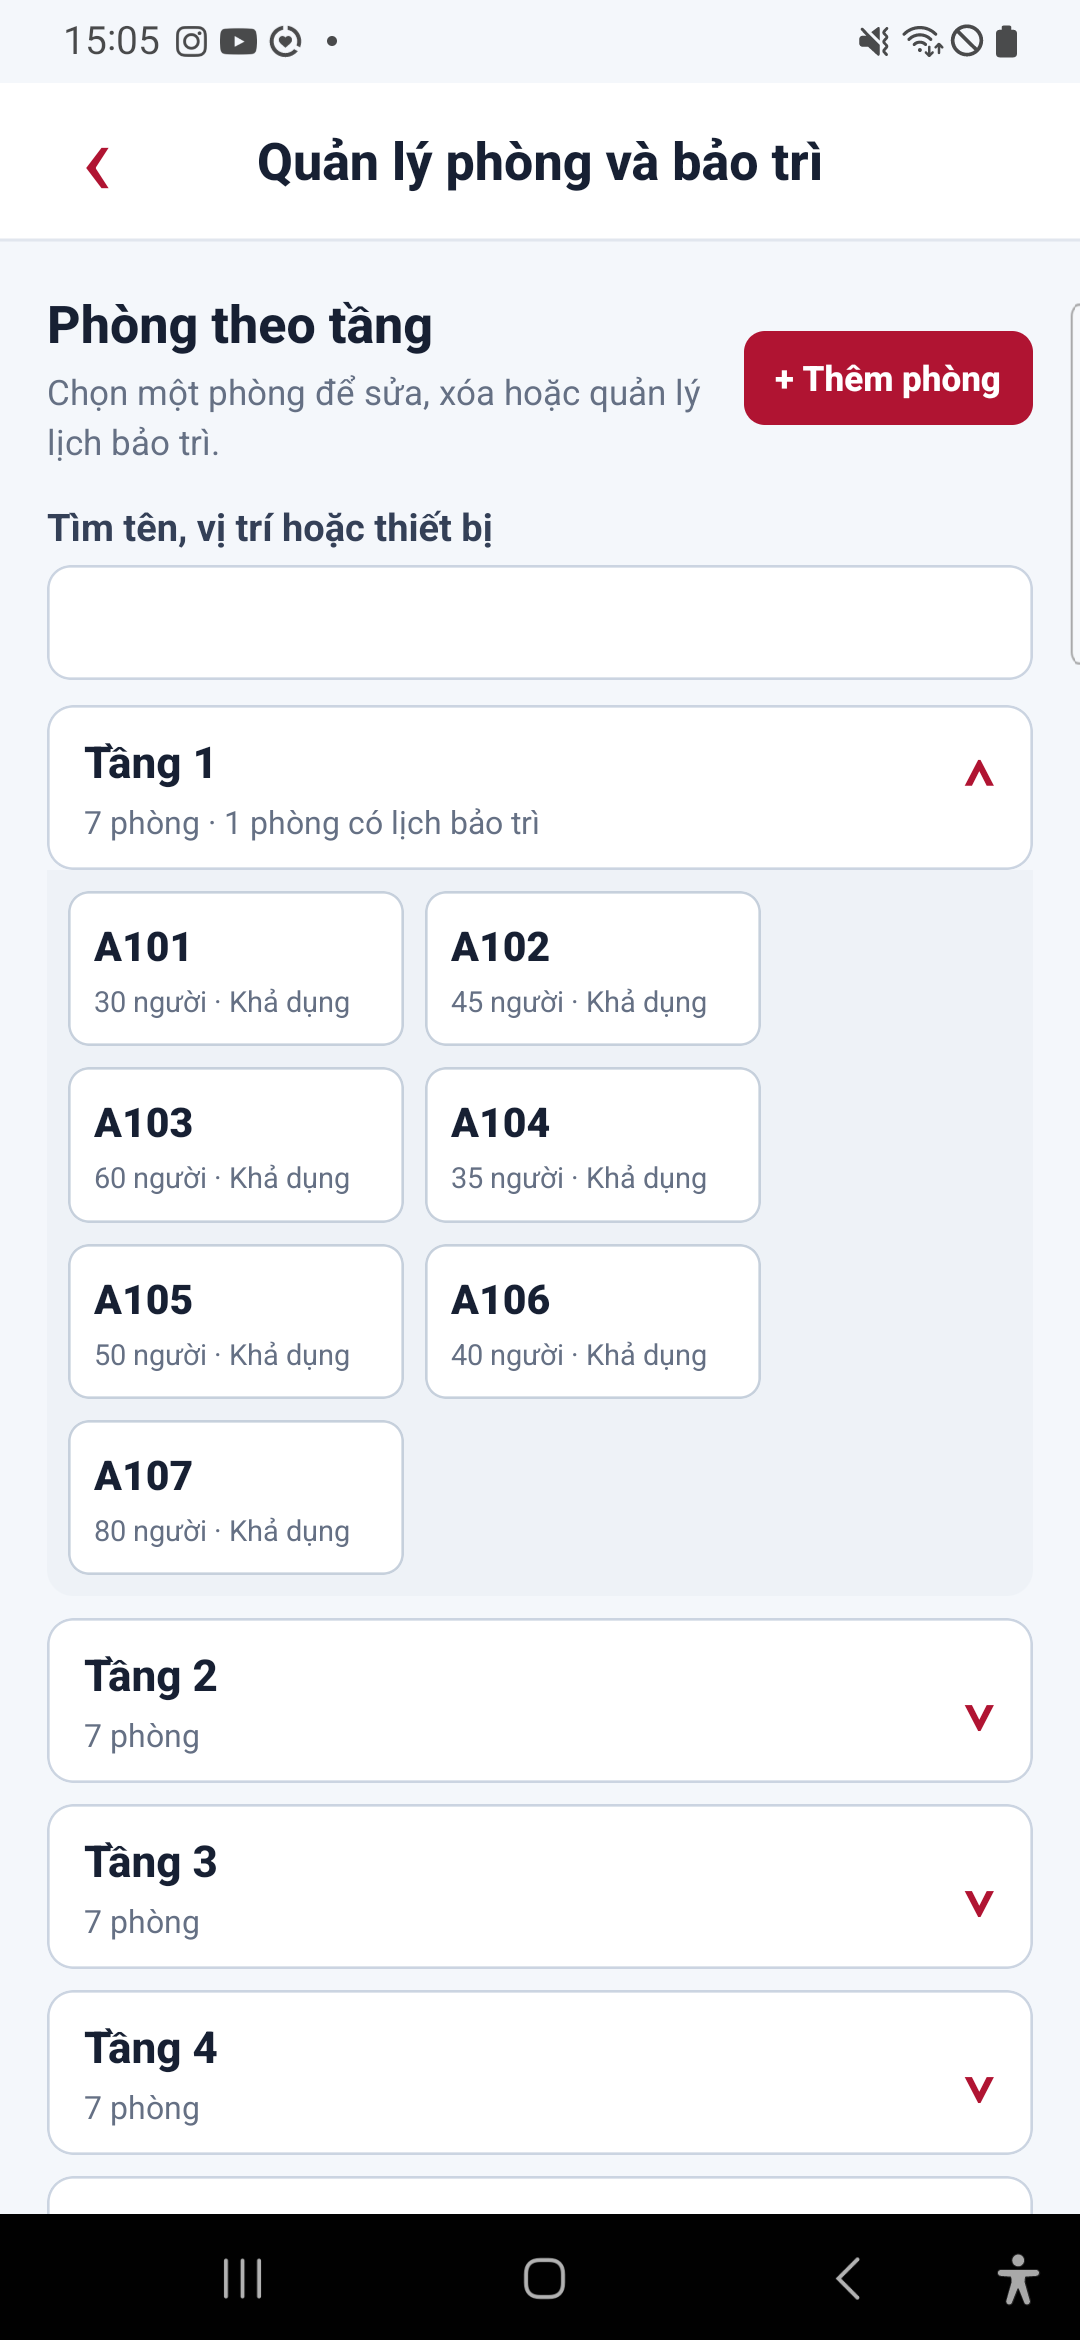
\includegraphics[width=\linewidth]{phong_tang_mot_hien_tai.png}
  \caption{Phòng thuộc tầng 1}
\end{subfigure}
\hfill
\begin{subfigure}[t]{0.43\textwidth}
  \centering
  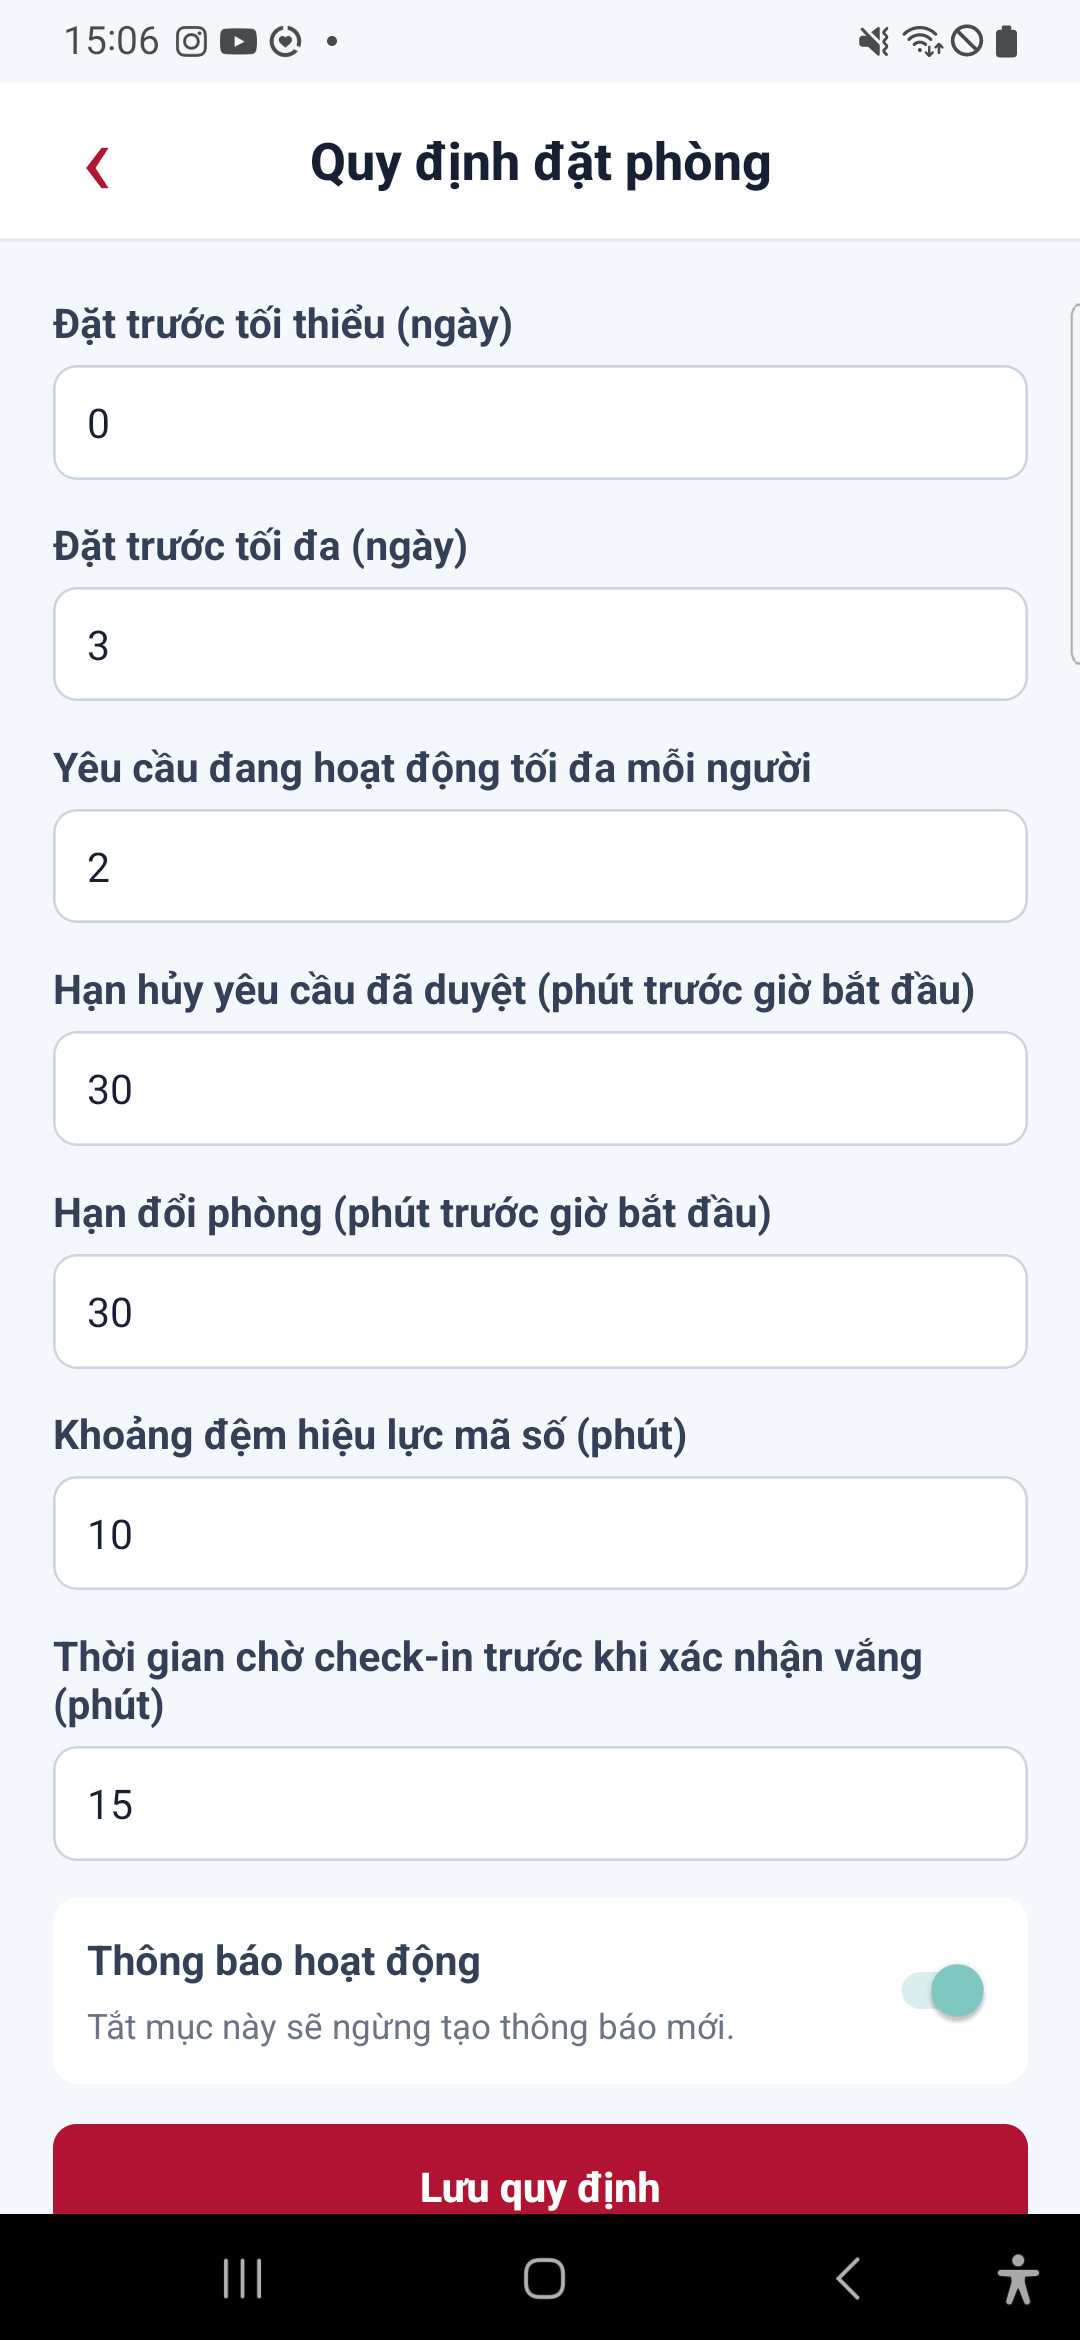
\includegraphics[width=\linewidth]{cau_hinh_hien_tai.png}
  \caption{Cấu hình quy tắc đặt phòng}
\end{subfigure}
\caption{Giao diện quản lý phòng và cấu hình nghiệp vụ}
\label{fig:current-admin}
\end{figure}



\chapter{QUY TRÌNH VÀ KỊCH BẢN KIỂM THỬ}
\label{chapter:Testing}
\section{Mục tiêu và phương pháp kiểm thử}

Ứng dụng được kiểm thử bằng các \textbf{kịch bản đầu cuối trên điện thoại thật}: cài bản Release từ APK, thao tác trực tiếp trên màn hình ở cả hai vai trò Admin và User, rồi đối chiếu kết quả với quy tắc nghiệp vụ \cite{istqb}.

Kịch bản bao gồm luồng nghiệp vụ chính, các giá trị biên (cửa sổ đặt 1--3 ngày, sức chứa, giới hạn yêu cầu, thời gian ân hạn) và chuyển trạng thái booking (Hình \ref{fig:state}). Chỉ bản build đạt bộ Jest \cite{jest} mới được đưa lên thiết bị.

\section{Môi trường kiểm thử trên thiết bị}

Các kịch bản nhiều vai trò được thực hiện bằng cách đăng nhập luân phiên Admin và User trên cùng một máy; các quy tắc theo thời gian được kiểm tra bằng cách chỉnh ngày giờ thiết bị.

\begin{table}[H]
\centering
\caption{Môi trường kiểm thử trên thiết bị thực tế}
\label{tab:env}
\small
\begin{tabularx}{\textwidth}{>{\raggedright\arraybackslash}p{3.6cm} X}
\toprule
\textbf{Hạng mục} & \textbf{Cấu hình} \\
\midrule
Thiết bị & Samsung Galaxy M21 (SM-M215F), Android \\
Bản cài đặt & \path{app-release.apk} build từ mã nguồn, cài bằng \texttt{adb install -r} \\
Công cụ theo dõi & \texttt{adb logcat} lọc lỗi \texttt{AndroidRuntime}, \texttt{ReactNativeJS}; ảnh chụp màn hình làm bằng chứng \\
Dữ liệu ban đầu & Xóa dữ liệu ứng dụng để về 56 phòng mẫu (8 tầng $\times$ 7 phòng), tài khoản \texttt{admin/1}, \texttt{user/2} \\
Cấu hình mặc định & Đặt trước 1--3 ngày, tối đa 2 yêu cầu, hủy trước 30 phút, ân hạn PIN 10 phút, no-show 15 phút \\
Mạng & Wi-Fi bật/tắt để kiểm thử trường hợp mất kết nối; OneIoT \texttt{oneiot.com.vn:2111} (MQTT/TLS) \\
\bottomrule
\end{tabularx}
\end{table}

\section{Quy trình kiểm thử trên thiết bị}

Quy trình gồm năm bước, lặp lại sau mỗi bản APK sửa lỗi, như Hình \ref{fig:testprocess}.

\begin{figure}[H]
\centering
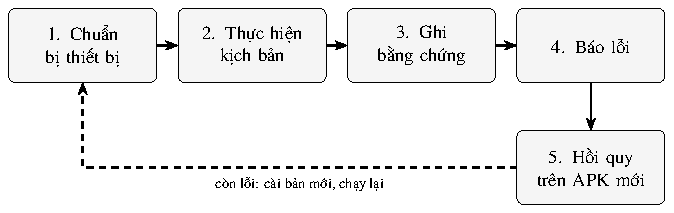
\includegraphics[width=0.98\textwidth]{quy_trinh_kiem_thu.pdf}
\caption{Quy trình kiểm thử trên thiết bị thực tế}
\label{fig:testprocess}
\end{figure}

Mỗi lỗi được ghi kèm kịch bản liên quan, các bước tái hiện, ảnh chụp màn hình và mức độ: \textit{Nghiêm trọng} (sai dữ liệu, chặn luồng chính), \textit{Cao} (sai quy tắc nghiệp vụ), \textit{Trung bình} (thiếu kiểm tra đầu vào) và \textit{Thấp} (giao diện). Lỗi chỉ được đóng khi kịch bản đạt trên bản APK mới.

\section{Kịch bản kiểm thử trên thiết bị}
\label{section:testcases}

Bảng \ref{tab:testcases} trình bày mười hai kịch bản; cột ``Lỗi'' tham chiếu tới Bảng \ref{tab:bugs}.

{\small
\begin{longtable}{>{\raggedright\arraybackslash}p{1.2cm} >{\raggedright\arraybackslash}p{5.9cm} >{\raggedright\arraybackslash}p{4.2cm} >{\centering\arraybackslash}p{1.1cm}}
\caption{Kịch bản kiểm thử đầu cuối trên thiết bị thực tế}\label{tab:testcases}\\
\toprule
\textbf{Mã} & \textbf{Các bước trên thiết bị} & \textbf{Kết quả mong đợi} & \textbf{Lỗi} \\
\midrule
\endfirsthead
\toprule
\textbf{Mã} & \textbf{Các bước trên thiết bị} & \textbf{Kết quả mong đợi} & \textbf{Lỗi} \\
\midrule
\endhead
\bottomrule
\endfoot
KB-01 & \textbf{Cài đặt và khởi động.} (1) Cài APK bằng \texttt{adb install -r}; (2) rút cáp, buộc dừng ứng dụng; (3) mở lại từ màn hình chính. & Ứng dụng mở màn hình đăng nhập, không cần Metro; logcat không có lỗi crash. & -- \\
\addlinespace
KB-02 & \textbf{Đăng nhập theo vai trò.} (1) Đăng nhập \texttt{admin/1}; (2) đăng xuất, đăng nhập \texttt{user/2}; (3) nhập sai mật khẩu. & (1) Chế độ quản trị viên; (2) chế độ người dùng; (3) báo sai thông tin. Màn hình không có chữ thừa. & L03 \\
\addlinespace
KB-03 & \textbf{Đăng ký và khôi phục mật khẩu.} (1) Chọn Đăng ký, bỏ trống mã khôi phục; (2) nhập đủ, tạo \texttt{teacher01}; (3) đăng ký lại tên \texttt{teacher01}; (4) Quên mật khẩu, nhập mã khôi phục, đặt mật khẩu mới; (5) đăng nhập bằng mật khẩu mới. & (1) Cảnh báo trường bắt buộc có dấu (*); (2) tạo thành công; (3) báo trùng tên; (4)--(5) đăng nhập được, mật khẩu cũ bị từ chối. & L02 L03 L04 \\
\addlinespace
KB-04 & \textbf{Hồ sơ cá nhân.} (1) User mở Thông tin cá nhân, sửa họ tên, email, số điện thoại, nhấn Lưu; (2) đóng hẳn ứng dụng rồi mở lại; (3) đăng nhập Admin, mở Quản lý user xem tài khoản đó. & Thông tin được giữ sau khi mở lại; Admin thấy cùng thông tin; User không thay đổi được vai trò của mình. & L05 L14 \\
\addlinespace
KB-05 & \textbf{Tìm phòng trên sơ đồ tầng.} (1) User mở Tìm phòng, chọn ngày mai 08:00--09:00; (2) nhập sức chứa tối thiểu 45; (3) chọn thiết bị Máy chiếu; (4) lần lượt chọn tầng T1--T8. & Mọi phòng $\geq$ 45 chỗ có máy chiếu được tô xanh, kể cả phòng đúng 45 chỗ; phòng không khớp được làm mờ. & L06 L07 \\
\addlinespace
KB-06 & \textbf{Đặt phòng và phê duyệt.} (1) User chọn phòng A102, ngày mai 09:00--11:00, bỏ trống Mục đích sử dụng, nhấn Gửi; (2) nhập ``Họp môn đồ án'', gửi lại; (3) đăng nhập Admin, mở Quản lý mượn phòng, duyệt; (4) đăng nhập User, mở Lịch đặt. & (1) Cảnh báo tại trường Mục đích; (2) yêu cầu ở trạng thái Chờ duyệt; (3) Admin thấy huy hiệu và thông báo mới; (4) User thấy Đã duyệt và thông báo màu xanh. & L09 L11 L12 \\
\addlinespace
KB-07 & \textbf{Quy tắc đặt phòng.} (1) User đặt phòng cho hôm nay và cho 4 ngày sau; (2) tạo yêu cầu thứ ba khi đã có hai; (3) đăng nhập \texttt{teacher01}, đặt A102 cùng khung giờ ở KB-06; (4) Admin mở Cấu hình nghiệp vụ, đổi tối đa thành 3; User đặt lại bước (2). & (1)--(3) bị từ chối với thông báo đúng quy tắc; (4) sau khi đổi cấu hình, yêu cầu thứ ba được tạo. & -- \\
\addlinespace
KB-08 & \textbf{Đặt lặp hàng tuần.} (1) User bật Lặp hàng tuần, 4 tuần, gửi yêu cầu; (2) mở Lịch đặt xem chuỗi; (3) Admin duyệt cả chuỗi; (4) User hủy các lượt tương lai. & Hiển thị đủ 4 lượt với ngày, giờ và trạng thái từng tuần; duyệt và hủy áp dụng cho cả chuỗi, đồng bộ giữa hai vai trò. & L10 L14 \\
\addlinespace
KB-09 & \textbf{Quản lý phòng và bảo trì.} (1) Admin mở Quản lý phòng, thêm phòng mới ở tầng 7; (2) lên lịch bảo trì một phòng vào ngày mai; (3) User tìm phòng ngày mai; (4) Admin xóa phòng đang có booking đã duyệt. & (1) Phòng mới xuất hiện trên sơ đồ tầng 7; (3) phòng bảo trì màu xám, không đặt được; (4) từ chối xóa. & L08 L13 \\
\addlinespace
KB-10 & \textbf{Báo sự cố khi đang dùng phòng.} (1) Chỉnh giờ thiết bị vào giữa phiên đã duyệt của User; (2) User mở booking, chọn Báo sự cố, nhập lý do; (3) Admin mở Quản lý phòng. & Admin nhận thông báo; tầng và phòng liên quan tô vàng; Admin tiếp nhận và lên lịch bảo trì được. & -- \\
\addlinespace
KB-11 & \textbf{Khóa cơ/thẻ từ và điểm danh.} (1) Với booking đã duyệt ở phòng khóa cơ, User đề xuất giờ nhận khóa; (2) Admin đề xuất giờ và địa điểm khác; (3) User chấp nhận; (4) chỉnh giờ vào phiên, Admin xác nhận có mặt; (5) với booking khác không check-in, chỉnh giờ qua 15 phút sau giờ bắt đầu, Admin ghi vắng mặt. & (3) Hai bên thấy lịch đã thống nhất; (4) booking có check-in; (5) trước 15 phút bị từ chối, sau 15 phút chuyển Vắng mặt và khung giờ được giải phóng. & -- \\
\addlinespace
KB-12 & \textbf{Khóa số và OneIoT.} (1) Admin cho phép đặt cùng ngày, gắn SmartLock vào A101; (2) User đặt A101 hôm nay khi phiên đã bắt đầu, Admin duyệt; (3) tắt Wi-Fi, User tạo mã tạm thời; (4) bật Wi-Fi, Admin nhập token Tools, nhấn Kiểm tra kết nối; (5) chuyển ứng dụng xuống nền. & (2) Duyệt được vì phiên chưa kết thúc; (3) mã 7 chữ số hiện ngay, trạng thái chờ gửi; (4) kết nối thành công, lệnh tự gửi; (5) phiên OneIoT tự ngắt, token không còn lưu. & -- \\
\end{longtable}
}

\section{Kết quả kiểm thử và lỗi đã phát hiện}

Bảng \ref{tab:results} tổng hợp kết quả trên Samsung M21.

\begin{table}[H]
\centering
\caption{Kết quả thực hiện kịch bản trên thiết bị}
\label{tab:results}
\small
\begin{tabularx}{\textwidth}{>{\raggedright\arraybackslash}p{1.2cm} >{\raggedright\arraybackslash}p{2.4cm} X}
\toprule
\textbf{Mã} & \textbf{Kết quả} & \textbf{Ghi chú} \\
\midrule
KB-01 & Đạt & Cài đặt, khởi động lại không cần Metro; 0 lỗi crash trong logcat \\
KB-02 & Đạt, có góp ý & Điều hướng đúng vai trò; còn chữ thừa trên màn hình đăng nhập (L03) \\
KB-03 & Không đạt & Thiếu đánh dấu bắt buộc, mã khôi phục chưa bắt buộc, lỗi tạo tài khoản (L02--L04) \\
KB-04 & Không đạt & Chưa kiểm tra quyền khi sửa hồ sơ, thông tin không đồng bộ (L05, L14) \\
KB-05 & Không đạt & Lọc sức chứa 45 chỉ hiện phòng 40 chỗ; chưa chọn từng thiết bị (L06, L07) \\
KB-06 & Không đạt & Thiếu cảnh báo Mục đích; lỗi đặt phòng phía server và lỗi khi duyệt (L09, L11, L12) \\
KB-07 & Đạt & Các quy tắc cửa sổ đặt, trùng lịch, giới hạn yêu cầu hoạt động đúng \\
KB-08 & Không đạt & Lịch sử chỉ hiện ngày đầu của chuỗi; đặt lặp không đồng bộ (L10, L14) \\
KB-09 & Không đạt & Không thêm được phòng; trạng thái đặt giờ không đồng bộ; nút Xóa thiếu lọc (L08, L13) \\
KB-10 & Đạt & Báo sự cố và tô vàng phòng hoạt động đúng \\
KB-11 & Đạt & Thỏa thuận nhận khóa, check-in, no-show đúng ân hạn \\
KB-12 & Đạt một phần & Lệnh đã gửi tới OneIoT; chưa kiểm chứng khóa thật mở bằng mã \\
\bottomrule
\end{tabularx}
\end{table}

Các lỗi phát hiện được tổng hợp ở Bảng \ref{tab:bugs}.

{\small
\begin{longtable}{>{\raggedright\arraybackslash}p{0.9cm} >{\raggedright\arraybackslash}p{2.8cm} >{\raggedright\arraybackslash}p{7.0cm} >{\raggedright\arraybackslash}p{1.9cm}}
\caption{Danh sách lỗi và vấn đề đã báo cho nhóm}\label{tab:bugs}\\
\toprule
\textbf{Mã} & \textbf{Module} & \textbf{Mô tả} & \textbf{Mức độ} \\
\midrule
\endfirsthead
\toprule
\textbf{Mã} & \textbf{Module} & \textbf{Mô tả} & \textbf{Mức độ} \\
\midrule
\endhead
\bottomrule
\endfoot
L01 & Giao diện & Cần sửa logo và màu sắc & Thấp \\
L02 & auth, profile & Thiếu Email, Mã nhân viên; trường bắt buộc chưa có dấu (*) & Trung bình \\
L03 & auth & Cập nhật Database; chữ thừa trên màn hình đăng nhập; mã khôi phục phải bắt buộc & Trung bình \\
L04 & auth & Xung đột khi đăng ký; lỗi tạo tài khoản liên quan Database & Nghiêm trọng \\
L05 & profile & Cập nhật thông tin cá nhân chưa kiểm tra Role/Quyền & Cao \\
L06 & Phòng & Thiết bị chưa chọn được từng mục & Trung bình \\
L07 & Phòng & Tìm theo sức chứa bỏ qua giới hạn: chọn 45 chỉ hiển thị 40 & Cao \\
L08 & Phòng & Nút Xóa cần bộ lọc tự động & Thấp \\
L09 & booking & ``Mục đích sử dụng'' chưa cảnh báo khi bỏ trống & Trung bình \\
L10 & booking & Lịch sử đặt theo tuần chỉ hiển thị ngày đầu tiên & Cao \\
L11 & booking & Bug liên quan server khi đặt phòng & Nghiêm trọng \\
L12 & booking & Lỗi trong quá trình duyệt & Cao \\
L13 & Phòng, bảo trì & Không thêm được phòng; trạng thái ``Đặt giờ phòng không đồng bộ'' & Nghiêm trọng \\
L14 & Đồng bộ dữ liệu & Đặt phòng và phê duyệt, thông tin cá nhân và tài khoản, đặt lịch hàng tuần không đồng bộ giữa các chức năng & Nghiêm trọng \\
\end{longtable}
}

Bốn lỗi Nghiêm trọng (L04, L11, L13, L14) đều liên quan đến đồng bộ dữ liệu và cần được ưu tiên xử lý, tiếp đến là các lỗi sai quy tắc nghiệp vụ, cuối cùng là giao diện. 

\chapter*{KẾT LUẬN}
\addcontentsline{toc}{chapter}{KẾT LUẬN}
\markboth{KẾT LUẬN}{}

Nhóm đã hoàn thành MVP của RoomHub: một ứng dụng Android chạy độc lập, bao phủ đầy đủ vòng đời mượn phòng từ tìm phòng trên sơ đồ tầng, đặt đơn lẻ hoặc lặp tuần, phê duyệt và đổi phòng, đến cấp quyền truy cập bằng khóa cơ/thẻ từ hoặc mật khẩu tạm thời. Mã nguồn được tổ chức thành mười module có ranh giới rõ, quy tắc nghiệp vụ tập trung ở lớp dịch vụ và được kiểm thử tự động. Quy trình kiểm thử năm bước cùng 12 kịch bản đầu cuối trên thiết bị thực tế đã phát hiện 14 nhóm vấn đề, trong đó lỗi đồng bộ dữ liệu là trọng tâm cần xử lý.

Hướng phát triển tiếp theo gồm: (i) bật đồng bộ qua booking server để dùng chung dữ liệu trên nhiều thiết bị và khắc phục nhóm lỗi đồng bộ; (ii) kiểm chứng đầu cuối với SmartLock thật; (iii) bổ sung QR check-in/check-out, thống kê mức sử dụng phòng và gợi ý phòng nâng cao.


% ===================================================
\cleardoublepage
\renewcommand\bibname{TÀI LIỆU THAM KHẢO}
\phantomsection\addcontentsline{toc}{chapter}{TÀI LIỆU THAM KHẢO}
\begin{thebibliography}{9}
\bibitem{reactnative} Meta Platforms, ``React Native -- Learn once, write anywhere.'' \url{https://reactnative.dev/docs/getting-started}. Truy cập 10/2026.
\bibitem{asyncstorage} React Native Community, ``Async Storage -- An asynchronous, persistent, key-value storage system for React Native.'' \url{https://react-native-async-storage.github.io/async-storage/}. Truy cập 10/2026.
\bibitem{springboot} VMware Tanzu, ``Spring Boot Reference Documentation.'' \url{https://docs.spring.io/spring-boot/}. Truy cập 10/2026.
\bibitem{mqtt} OASIS, ``MQTT Version 3.1.1, OASIS Standard,'' 2014. \url{https://docs.oasis-open.org/mqtt/mqtt/v3.1.1/mqtt-v3.1.1.html}.
\bibitem{onem2m} oneM2M Partners, ``oneM2M TS-0010: MQTT Protocol Binding.'' \url{https://www.onem2m.org/technical/published-specifications}. Truy cập 10/2026.
\bibitem{istqb} ISTQB, ``Certified Tester Foundation Level Syllabus v4.0,'' 2023. \url{https://www.istqb.org/}.
\bibitem{jest} OpenJS Foundation, ``Jest -- Delightful JavaScript Testing.'' \url{https://jestjs.io/docs/getting-started}. Truy cập 10/2026.
\end{thebibliography}

\appendixpage
\appendices
\addappheadtotoc
\titleformat{\chapter}[hang]{\centering\bfseries}{\thechapter.\ }{0pt}{}[]
\titlespacing*{\chapter}{0pt}{-20pt}{14pt}
\titlecontents{chapter}[0.0cm]{\bfseries\vspace{0.3cm}}{{\bfseries \thecontentslabel.\ }}{}{\titlerule*[0.3pc]{.}\contentspage}

\chapter{TỔNG THỂ THÀNH PHẦN DỰ ÁN}
\label{appendix:components}

\section{Cấu trúc kho mã nguồn}

Kho mã nguồn \url{https://github.com/xwomen1/classroom-booking} được tổ chức như Đoạn mã \ref{lst:tree}. Kho chỉ lưu mã nguồn cần thiết; tệp APK, bộ nhớ đệm, \texttt{node\_modules} và thư mục build không được đưa lên Git, mỗi thành viên tự build sau khi clone.

\begin{code}[H]
\caption{Cấu trúc thư mục chính}\label{lst:tree}
\begin{Verbatim}[breaklines, breakanywhere, frame=single, framesep=2mm, rulecolor=\color{gray!50}, fontsize=\footnotesize]
classroom-booking/
|-- README.md                    Hướng dẫn clone, build, cài APK
|-- du_an_dat_phong.tex/.pdf     Đề xuất dự án
|-- workflow_booking_app.tex/.pdf Workflow nghiệp vụ
|-- hien_trang_trien_khai.tex/.pdf Hiện trạng triển khai
|-- code/
|   |-- booking_classroom/       Ứng dụng React Native (Android)
|   |   |-- App.tsx              Điểm vào, điều hướng theo vai trò
|   |   |-- src/core/            api client, cờ cấu hình, storage
|   |   |-- src/shared/          component dùng chung
|   |   |-- src/modules/         10 module nghiệp vụ
|   |   |-- __tests__/           36 ca kiểm thử Jest
|   |   |-- android/.../OneIoTMqttPackage.kt     MQTT/TLS tới OneIoT
|   |   |-- android/.../PriorityNotificationPackage.kt  banner
|   |   |-- docs/, evidence/     sơ đồ luồng, ảnh kiểm tra thiết bị
|   |   `-- scripts/             build Debug/Release (PowerShell)
|   `-- booking-server/          Spring Boot + H2
|       `-- src/main/java/com/bookingclassroom/server/
|           ApiController, BookingService, SessionAuthFilter,
|           ApiExceptionHandler, DataSeeder, Domain
|-- tunghv2/                     Giả lập SmartLock (Python)
`-- tunghv3/                     Gateway HTTP-MQTT cũ (Python)
\end{Verbatim}
\end{code}

\section{Build và cài đặt}

Ứng dụng được build và cài đặt bằng các lệnh trong Đoạn mã \ref{lst:build}. Bản Release chạy độc lập sau khi cài, không cần Metro, cáp USB hay booking server.

\begin{code}[H]
\caption{Build và cài đặt bản Release}\label{lst:build}
\begin{Verbatim}[breaklines, breakanywhere, frame=single, framesep=2mm, rulecolor=\color{gray!50}, fontsize=\footnotesize]
git clone https://github.com/xwomen1/classroom-booking.git
cd classroom-booking/code/booking_classroom
npm ci
npm run build:android:release
adb install -r ./android/app/build/outputs/apk/release/app-release.apk
npm test        # chạy bộ kiểm thử Jest
npm run lint    # kiểm tra ESLint
\end{Verbatim}
\end{code}

\section{Tổng hợp tài liệu và phụ lục}

Bảng \ref{tab:docs} tóm tắt các tài liệu đi kèm dự án và nơi chúng được tham chiếu trong báo cáo.

\begin{table}[H]
\centering
\caption{Tài liệu đi kèm dự án}
\label{tab:docs}
\small
\begin{tabularx}{\textwidth}{>{\raggedright\arraybackslash}p{4.6cm} X}
\toprule
\textbf{Tài liệu} & \textbf{Nội dung} \\
\midrule
\path{du_an_dat_phong.pdf} & Đề xuất dự án, phạm vi, tiêu chí kiểm chứng \\
\path{workflow_booking_app.pdf} & Workflow nghiệp vụ đặt phòng, phê duyệt, bàn giao \\
\path{hien_trang_trien_khai.pdf} & Hiện trạng các chức năng đã kiểm tra \\
\path{evidence/device-verification.txt} & Nhật ký kiểm tra trên Samsung M21 \\
\path{RoomHub_final.pptx} & Slide trình bày sản phẩm \\
Phụ lục \ref{appendix:prompt} & Prompt sử dụng trong quá trình phát triển \\
\bottomrule
\end{tabularx}
\end{table}


\chapter{PROMPT SỬ DỤNG TRONG QUÁ TRÌNH PHÁT TRIỂN}
\label{appendix:prompt}
Nhóm sử dụng trợ lý lập trình để hỗ trợ phân tích yêu cầu, rà soát mã, đề xuất kiểm thử và soạn tài liệu. Trợ lý không tự quyết định phạm vi sản phẩm hoặc xác nhận một chức năng đã hoàn thành. Mọi thay đổi đều phải được thành viên phụ trách đọc lại, chạy kiểm thử và kiểm tra trên nhánh làm việc trước khi hợp nhất.

\section{Nguyên tắc sử dụng}

\begin{enumerate}
  \item Nêu rõ mục tiêu, module, tệp liên quan và quy tắc nghiệp vụ cần giữ.
  \item Giới hạn phạm vi thay đổi để tránh tác động ngoài ý muốn tới module khác.
  \item Yêu cầu chỉ ra giả định và đối chiếu với mã nguồn trước khi sửa.
  \item Luôn kèm bước kiểm tra phù hợp như Jest, TypeScript, ESLint, kiểm thử tích hợp hoặc build APK.
  \item Không đưa token, mật khẩu thật hoặc dữ liệu nhạy cảm vào mã nguồn và lịch sử Git.
  \item Chỉ commit sau khi xem lại diff; chỉ push khi người phụ trách cho phép.
\end{enumerate}

\section{Các nhóm prompt tiêu biểu}

\begin{longtable}{>{\raggedright\arraybackslash}p{3.0cm}>{\raggedright\arraybackslash}p{10.0cm}}
\caption{Prompt tiêu biểu trong quá trình phát triển}\label{tab:prompts}\\
\toprule
\rowcolor{RoomHubLight}
\textbf{Mục đích} & \textbf{Nội dung rút gọn} \\
\midrule
\endfirsthead
\toprule
\rowcolor{RoomHubLight}
\textbf{Mục đích} & \textbf{Nội dung rút gọn} \\
\midrule
\endhead
\bottomrule
\endfoot
Phân tích nghiệp vụ & ``Đối chiếu yêu cầu đặt phòng với mã hiện tại; xác định thực thể, trạng thái và quy tắc còn thiếu. Không tự bổ sung yêu cầu chưa có căn cứ.'' \\
Tổ chức module & ``Sắp xếp mã theo module để các thành viên phát triển độc lập; chỉ rõ màn hình, dịch vụ, mô hình dữ liệu và API công khai của từng module.'' \\
Triển khai chức năng & ``Cài đặt luồng tạo PIN tạm thời: mã gồm 7 chữ số, thời hạn lấy từ lịch đặt, lưu cục bộ trước và chỉ gửi khi phiên OneIoT đã kết nối.'' \\
Rà soát đồng bộ & ``So sánh repository cục bộ với REST API; tìm sai khác về quyền, trạng thái và cấu trúc dữ liệu; kiểm thử bằng Spring Boot/H2 cục bộ khi máy chủ thật chưa hoạt động.'' \\
Kiểm thử & ``Viết hoặc cập nhật ca kiểm thử cho quy tắc vừa sửa; chạy Jest, TypeScript và ESLint; báo rõ lệnh, kết quả và giới hạn chưa kiểm chứng.'' \\
Hợp nhất nhánh & ``Đọc toàn bộ xung đột; ưu tiên thay đổi mới của nhánh được hợp nhất, nhưng giữ chức năng hiện có nếu nhánh đó làm mất endpoint hoặc quy tắc đã triển khai.'' \\
Build thiết bị & ``Build APK Release với chế độ cục bộ, cài lên điện thoại thật, mở ứng dụng, đăng nhập tài khoản trình diễn và kiểm tra log lỗi nghiêm trọng.'' \\
Rà soát tài liệu & ``Đối chiếu báo cáo với mã nguồn và kết quả kiểm thử; loại bỏ khẳng định không có bằng chứng; chuẩn hóa thuật ngữ, bảng biểu, hình và tham chiếu.'' \\
\end{longtable}

\section{Quy trình kiểm soát đầu ra}

Đầu ra từ trợ lý được kiểm soát qua bốn bước: (1) xem danh sách tệp thay đổi; (2) đọc diff và đối chiếu quy tắc nghiệp vụ; (3) chạy bộ kiểm tra tương ứng; (4) kiểm tra thủ công luồng chính trên bản Release nếu thay đổi ảnh hưởng giao diện hoặc tích hợp thiết bị. Nếu một bước không đạt, thay đổi được sửa tại nhánh làm việc và kiểm tra lại trước khi commit.

Các nội dung chưa thể kiểm chứng, chẳng hạn máy chủ thật đang tắt hoặc khóa vật lý chưa sẵn sàng, phải được ghi rõ là giới hạn. Báo cáo không coi kết quả mô phỏng là bằng chứng cho hoạt động của hạ tầng thật.
\end{document}
